\documentclass[10pt]{article}
\usepackage[a4paper,margin=22mm]{geometry}
\usepackage{iftex}
\ifXeTeX\usepackage{fontspec}\else\usepackage[T1]{fontenc}\usepackage[utf8]{inputenc}\usepackage{lmodern}\fi
\usepackage{textcomp}
\usepackage{amsmath,amssymb,amsthm}
\usepackage{graphicx,booktabs,array,xcolor,longtable}
\usepackage[font=small,labelformat=empty,justification=justified,singlelinecheck=false]{caption}
\usepackage{microtype}
\usepackage[numbers,super,sort&compress]{natbib}
\usepackage[hidelinks]{hyperref}
\usepackage{xurl}
\setlength{\parskip}{0.35em}
\setlength{\parindent}{0pt}
\renewcommand{\bibnumfmt}[1]{#1.}
\makeatletter\setlength{\@fptop}{0pt}\setlength{\@fpsep}{12pt}\setlength{\@fpbot}{0pt plus 1fil}\makeatother
\renewcommand{\topfraction}{0.92}\renewcommand{\textfraction}{0.06}\renewcommand{\floatpagefraction}{0.8}

\newcommand{\figlabel}[2]{\textbf{#1 $|$ #2}}
\newtheorem{proposition}{Proposition}
\newcommand{\notyet}{\bot}

\title{When the Check Is the Algorithm}
\author{Mostafa `Neo' Mohsenvand\\ {\small MIT Media Lab} \and Pouyan Jahangiri\\ {\small Independent researcher}}
\date{}

\begin{document}
\maketitle

\begin{abstract}
\noindent Looped neural networks learn algorithms and puzzles, but they train through their loops, for hours. CRAM, a
classical energy recently revived, fits to solved puzzles in milliseconds; what it learns, though, is a check tied to one
board size, with no place for quantities the answer does not show. We show that a check fitted at the answer can be the
algorithm itself. We complete each training answer with closures and counts, fit the zero-temperature
pair-attention check of our earlier work to it in one step, and keep the one condition a finished answer never
contradicts: every part rests on parts placed before it. Run cold from nothing, the check rebuilds the answer at any
size, and a search runs only where nothing is forced. One rule, fitted in about 20 milliseconds, solves all
412,786 Sudoku-Extreme puzzles and, unchanged, boards of $16\times16$ and $25\times25$. A maze rule that reads the cold run's own clock, in place of CRAM's hand-built distance layer, solves all 1,000
Maze-Hard mazes. All thirty CLRS-30 tasks are exact on the
official test and on held-out inputs of up to 1,024 nodes, fifteen of them from comparisons and
counts, thirteen with nothing supplied at all, each fitted in milliseconds to seconds on one CPU core, and one check serves five graph algorithms at once. The fitted rules are small tables with no size in
them, so finite checks prove the puzzle rules, and the checks of several algorithms, correct at every size. In the language of logic programming, the kept condition
turns an answer the check merely supports into the least model the check computes.
\end{abstract}

\section{Introduction}

Neural networks that apply one block again and again, in a loop, have learned to solve Sudoku, mazes and the textbook
algorithms of the CLRS-30 benchmark\cite{wang2025hrm,jolicoeur2025trm,velickovic2022clrs,bansal2022end}. They are
trained through their loops, and that is slow. On Sudoku-Extreme the strongest of them train for 1.2 to
9.0 hours on a GPU in CRAM's reproductions\cite{hoover2026classical}, from HRM to
TRMP\cite{wang2025hrm,jolicoeur2025trm,salvatori2026tiny,chen2026energy}. The looped attention blocks of our earlier paper needed
about an hour of GPU time for each CLRS-30 task\cite{mohsenvand2026zero}.

Hoover, Blayney and Whittington showed that much of this cost can be avoided\cite{hoover2026classical}. Their model,
CRAM, is the pairwise energy that Hopfield and Tank proposed for puzzles\cite{hopfield1985neural}, with its tables fitted
by pseudolikelihood\cite{besag1975statistical}: each cell of a solved board is predicted from the others, so training
needs no loop and no search. CRAM trains in 42 milliseconds and solves 99.996\% of
Sudoku-Extreme. Its authors name its two limits. Its costs belong to particular cells, so a model fitted at one board
size says nothing at another. And it has no place for a quantity the answer does not show: on Maze-Hard it needs a
hidden distance layer designed for the task, and learning such quantities in general is left open.

What a fit at a solved example learns is a check, a rule that each part of the answer satisfies given the rest. A check
is not yet an algorithm. At a finished answer every fact is in place, so facts may hold one another up in a circle, and
nothing in the fit asks whether the rule, started from nothing, would put them there. Logic programming names the gap
exactly: a finished answer the rules accept is a supported model; what the rules derive from nothing is their least
model; and the two coincide when the support has a direction\cite{clark1978negation,fages1994consistency}.

We give the check that direction, and it becomes the algorithm. We start from the cold layer of our earlier
paper\cite{mohsenvand2026zero} (Fig.~\ref{fig:arch}). Its state lives on pairs of items. It judges each pair $(a,b)$ through every third item
$k$, by the legs $(a,k)$ and $(k,b)$, and reads these witnesses at zero temperature: whether one exists, and how two
counts compare. Its rules attach to relations, never to positions, so they have no size in them. We fit its check at
finished answers, CRAM's way, in three steps.
\begin{itemize}
\setlength{\itemsep}{0pt}
\item \emph{Complete the answer from itself.} Closures and counts of the answer's own relations add what the answer
hides; a parent pointer, for instance, gives each node its depth.
\item \emph{Fit the check and keep every condition that held on all training answers.} Among them is the level
condition, that every part rests on parts placed before it. A finished answer never contradicts it, so a fit alone can
drop it.
\item \emph{Run the check cold.} From an empty state, apply the check and recompute the completion until nothing changes.
Where nothing is forced, as on hard puzzles, a search uses the check as its stop.
\end{itemize}

The check then trains like CRAM and runs like our looped layer (Fig.~\ref{fig:idea}). All thirty CLRS-30 tasks are
exact on the official test and on every held-out input, up to 1,024 nodes and 5,120 items,
the largest size per task in Table~\ref{tab:clrs}. Fifteen of them, among them breadth-first search, the minimum spanning
trees of Kruskal and Prim, longest common subsequence and both string matchers, are learned from their final answers
with comparisons and counts, thirteen with nothing supplied at all, each fitted in 18 ms to 4.1 s on one laptop core; the other fifteen read one quantity we supply,
such as the sum of a distance and an edge weight. The fitted rules read like the textbook: a node's breadth-first parent
is its lowest-numbered neighbour one level up. On CRAM's benchmarks, one rule fitted in about 20 milliseconds keeps
exactly the row, column and box relations of Sudoku. It solves all 412,786 Sudoku-Extreme puzzles with no
wrong answer, with 36,000 times fewer operations than CRAM (2,500 times with every comparison
counted), and solves larger boards unchanged. A maze
rule that reads the cold run's own clock, in place of a distance layer built for the task, solves every Maze-Hard maze,
and every maze we built on which CRAM's released model leaves the shortest path. The fitted rules are small tables with
no size in them, so finite checks prove the puzzle rules, and the checks of several algorithms, correct at every size
(Fig.~\ref{fig:cost} sets cost against reach). Read the same way, CRAM's released weights show its hidden distance
layer cooling, as it trains, towards the hard minimum that our cold layer reads.

\begin{figure}[tbp]
\centering
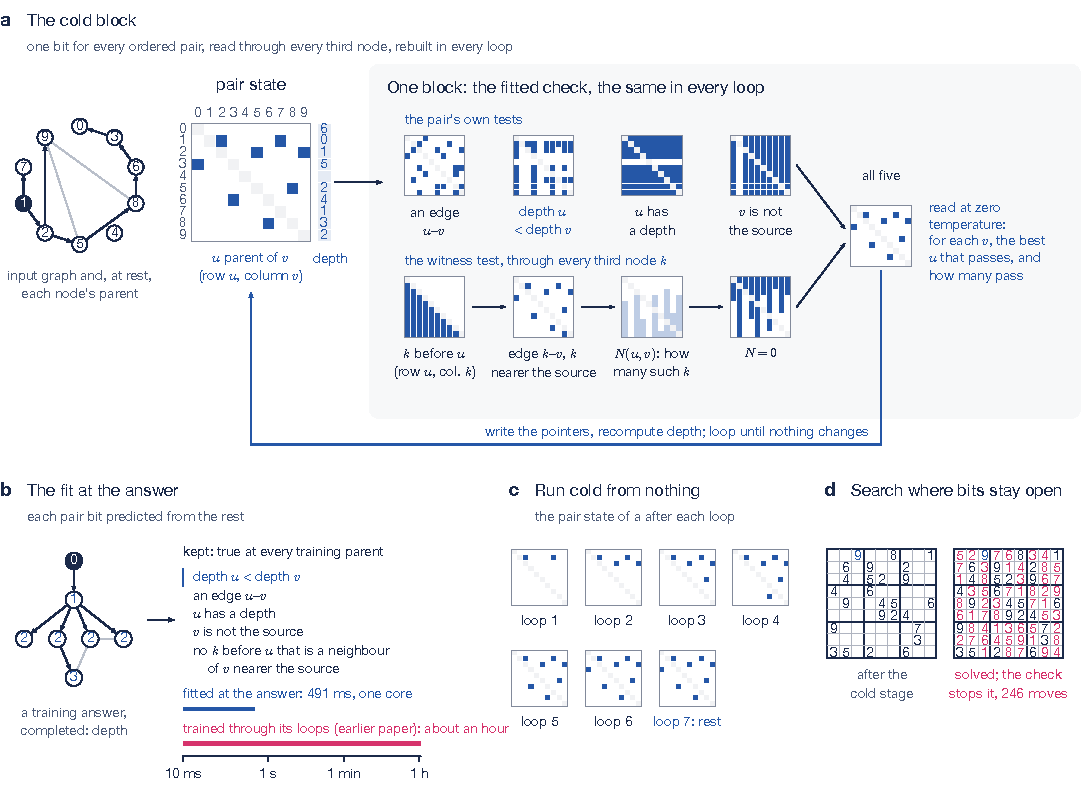
\includegraphics[width=\linewidth]{figures/fig_arch.pdf}
\caption[]{\figlabel{Fig. \thefigure}{The cold block, fitted at the answer.} One example throughout: the CLRS-30 breadth-first-search check,
fitted at the completed answer and run on a ten-node input of the benchmark's generator. Cobalt: the block's bits,
counts and pointers; rose: what it is set against, training through the loops (b) and the search (d). \textbf{a}, The
block. Its state is one bit for every ordered pair of nodes, ``$u$ is the parent of $v$'' (row $u$, column $v$; shown at
rest), beside a register completed from those bits, each node's depth (its number of ancestors). One loop of the block
is the fitted check, the same in every loop. It reads the pair's own tests (four bit tables) and one witness test
through every third node $k$: row $u$ of the first leg (``$k$ comes before $u$'') meets column $v$ of the second
(``$k$ is a neighbour of $v$ nearer the source''), giving $N(u,v)$, the exact number of such $k$, and the bit $N=0$.
Where all five hold, the check passes; the read at zero temperature keeps, for every $v$, the best-scoring $u$ that
passes and the number that pass (here one for every node). The pointers are written, the depths recomputed from them,
and the block runs again until nothing changes. Every table is computed by the fitted check on this input.
\textbf{b}, The fit at the answer: one of the 100 training answers (seven nodes), completed from
itself (each node's depth). Each pair bit is predicted from the rest, and the fit keeps every condition that held at
every training parent; this is the check of a, its first condition the level condition. It takes 491~ms
on one laptop core; our earlier paper's blocks, trained through their loops,
took about an hour of GPU time for each task (the general block's median, 64 minutes). \textbf{c}, The check run cold from nothing on the input of a: the pair state after each loop. Each loop settles
the nodes one step further from the source; the state stops changing at loop 7, where every parent is the answer's.
\textbf{d}, Where bits stay open, a search: the Sudoku-Extreme puzzle of Fig.~\ref{fig:puzzles}a after the cold stage (navy, given;
cobalt, set cold) and solved (rose, set by the search, which stops when the same check passes). Schematic: the
layouts of the graphs (the ring order of a, the rows by depth in b).}
\label{fig:arch}
\end{figure}

\begin{figure}[tbp]
\centering
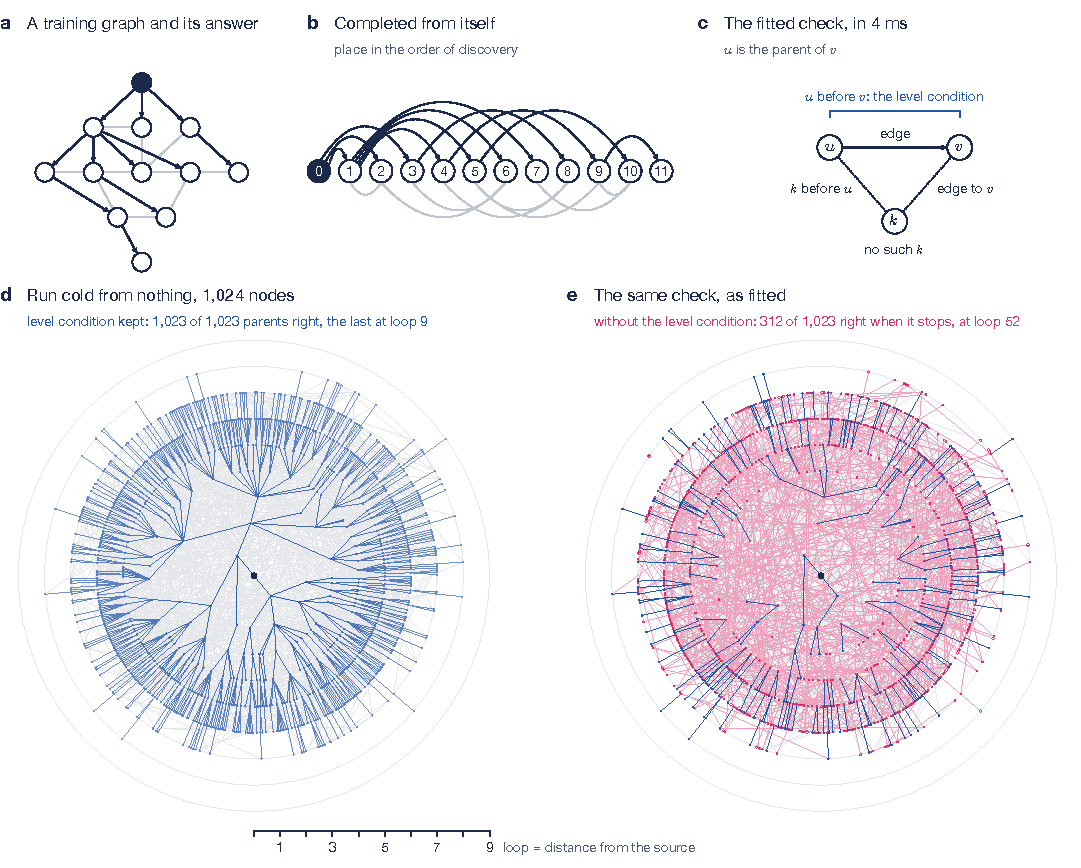
\includegraphics[width=\linewidth]{figures/fig1.pdf}
\caption[]{\figlabel{Fig. \thefigure}{The check is the algorithm.} Breadth-first search with queue-order parents (the textbook labelling), from one finished answer to a cold run on a graph 64
times larger than the largest training graph (16 nodes). Cobalt: the fitted check run cold with the level condition kept; rose: the same check as
fitted. \textbf{a}, One of the 30 training graphs (12 nodes) and its answer, each node's parent (arrows; the source
filled; grey, the graph's other edges). \textbf{b}, The completion, computed from the answer alone: each node's place in
the order of discovery, which is also its position on the line. Arcs above join each parent to its child and always
run left to right; arcs below are the other edges. \textbf{c}, The check the fit returned for ``$u$ is the parent of
$v$'', in 4 ms on one laptop core, drawn as the cold layer reads it: the pair $(u, v)$ joined by an edge, and a witness
test through a third node $k$, ``no neighbour $k$ of $v$ placed before $u$'' (the largest weights of the fit). The
bracket is the level condition, ``$u$ placed before $v$'': it held at every training parent, so a fit at the answer has
no reason to use it, and we keep it. \textbf{d}, The check run from ``not yet'' on a test graph of 1,024 nodes, with the
level condition kept: every node's parent is right, and each node is settled in the loop equal to its distance from the
source, the ring it sits on (scale below; the last at loop 9). \textbf{e}, The same check as fitted, on the same graph:
it settles 776 nodes in its first loop, 554 of them with a wrong parent (rose chords, from the parent named to the
node), and when it stops, at loop 52, 312 of the 1,023 parents are right (cobalt) and 49 nodes are unsettled (open
circles). Schematic: the node positions in a, b and the radial layout of d and e (the source at the centre, ring $r$ at
distance $r$, each subtree a wedge); the rings and their distances are data.}
\label{fig:idea}
\end{figure}

\section{Fitting a check at the answer}\label{sec:setting}

An example is an input $x$ on a set $V$ of $n$ items, together with its answer $y$. The input holds numbers on items
(keys, times, weights), relations on pairs of items (an edge, two letters that are the same) and numbers on pairs (edge
weights); numbers enter only through comparisons. The answer is a set of bits on items or on pairs. A pointer answer,
such as the parent tree of a search, is the pair bit $\pi(u,v)$, ``$u$ is the parent of $v$'', with $\pi(v,v)$ for a
root. Our state is the one of our cold layer\cite{mohsenvand2026zero}: bits and small whole numbers for every item and
every ordered pair, the answer included.

\subsection{Completing the answer}

An answer often hides what decided it. A parent tree does not show how deep each node lies, and the depth is what tells
a breadth-first parent from any other neighbour. We therefore add registers by two generic operations, closure and
counting. For a pointer answer,
\begin{equation}
\mathrm{anc}_y = \pi^{+}, \qquad \mathrm{depth}_y(v) = \#\{u \neq v : \mathrm{anc}_y(u,v)\},
\label{eq:completion}
\end{equation}
where $\pi^{+}$ is the transitive closure of the pointer, counted from the source: a node that the pointer does not
connect to the source receives the value $\notyet$, read ``not yet''. Comparisons treat $\notyet$ as later than every
number: for a number $a$, $a < \notyet$ and $\notyet > a$ hold (and so do $a \leq \notyet$ and $\notyet \geq a$), and
every other comparison with $\notyet$, including $\notyet$ against $\notyet$, is false. The other completions are of the
same two kinds. Three read the answer: the depth, the sum of the weights along the pointer, and, for the longest common
subsequence, the number of match arrows along the answer's own arrows. Two read the input: the bottleneck closure of the
edge weights (for each pair, the least possible largest weight on a path between them) and, for the string matchers, the
closure of ``the text and the pattern agree from here to the pattern's end''. We write $y^{+} = (y, \kappa(y))$ for the
completed answer. No step of any algorithm enters $\kappa$, and the same few operations serve every task.

\subsection{The check}

For a target bit on a pair $(u,v)$, the check is a conjunction of conditions drawn from one fixed family $\Phi$, built
from the input's types alone:
\begin{itemize}
\setlength{\itemsep}{0pt}
\item the pair's own comparisons: $r(u)$ against $r(v)$ ($<$, $\leq$, $=$, $\geq$, $>$) for item registers $r$ of the input
or the completion; one pair number against another on the same pair ($<$, $=$, $>$), such as an edge weight against the
bottleneck; the input relations between $u$ and $v$; and the item bits of $u$ and $v$;
\item witness tests through a third item, $\exists k \notin \{u,v\} : A(u,k) \wedge B(k,v)$, where a leg test is an
own-style test on the pair it joins, optionally a relation or pair-number comparison conjoined with a register
comparison, optionally with a bit of $k$; and pair-number tests through a third item, $\exists k \notin \{u,v\} :
B(k,v) \wedge N_1(k,v) \mathbin{\mathrm{op}} N_2(u,v)$;
\item for an item target $i$, comparisons of two counts, $\#\{k : A(k,i)\} < \#\{k : B(k,i)\}$ or $=$.
\end{itemize}
Each condition can enter a rule negated, and since $\notyet$ fails every comparison it enters, a negated comparison and
its strict counterpart agree on numbers but differ on $\notyet$. With $C \subset \Phi$ the conditions the fit chooses,
\begin{equation}
R(u,v) = \bigwedge_{\varphi \in C} \varphi(x, y^{+})(u,v), \qquad
\pi(v) = \operatorname*{arg\,max}_{u \,:\, R(u,v)} s(u,v),
\label{eq:check}
\end{equation}
where a score $s$ breaks ties among the candidates that pass; the self-pointer $u = v$, ``$v$ has no parent'', competes
with the others by its own rule and score. These are the reads of the cold layer (Fig.~\ref{fig:arch}): a witness test is
its existence read, a count comparison one of its verdict bits\cite{mohsenvand2026zero}. Nothing in $\Phi$ names a
position or a size, so a rule fitted on graphs of 16 nodes applies, unchanged, to graphs of a thousand.

\subsection{Fitting at the answer}

As CRAM does, we predict each bit of a training answer from the rest of the completed answer and the input, with no
loop. Because the answers are exact, we fit the rule of each bit as a conjunction, in two steps. We first keep every own
condition that held on all training positives and failed on at least $\max(10, 0.5\%)$ of the training rows,
\begin{equation}
K = \{\varphi \in \Phi_{\mathrm{own}} : \varphi(u,v) = 1 \text{ for every positive } (u,v) \text{ of every training answer}\},
\label{eq:kept}
\end{equation}
where $\Phi_{\mathrm{own}}$ holds the pair's own conditions. We then add conditions greedily, each true on every positive:
at each step, the one that rejects the most training negatives that still pass, until none passes. This is the classical
learner of a conjunction\cite{haussler1988quantifying}, and $C = K \cup G$, with $G$ the conditions it adds. A logistic
regression with an $\ell_1$ penalty over all of $\Phi$, the pseudolikelihood of each bit given the rest, supplies the
score $s$. A target's own completed value enters its register comparisons only as ``the other item is below me'' ($r(u) < r(v)$
with $r(v)$ the target's), so that it cannot read off the answer it is meant to produce. For breadth-first search, for example, the fit
chooses among 6,249 candidate conditions from 100 training answers.

The kept set $K$ is a safeguard. A condition true on every training positive cannot help to reject a negative that the
other conditions already reject, so a sparse or greedy fit has no reason to include it. One such condition is that the
parent lies below the child, $\mathrm{depth}(u) < \mathrm{depth}(v)$. It is true at every finished answer, and it is
the condition that matters on the way to one (Section~\ref{sec:theory}). It also makes ``$u$ is reached'' redundant,
since $\mathrm{depth}(u) < \mathrm{depth}(v)$ is false whenever $\mathrm{depth}(u) = \notyet$.

On puzzles, where every cell holds one of several values, we follow CRAM more closely (Methods). Pseudolikelihood with
an $\ell_1$ penalty chooses which relations between cells carry a cost, from a vocabulary of coordinate relations such
as ``same row'' and ``same block''. For each relation it keeps, we record, over all training answers, the range of the
number of related cells that hold a value. The check passes a board when every such count lies in its range.

\subsection{Running the check cold}

The cold run starts from the empty answer, with no pointer, no selection and every register at $\notyet$, and applies
the check to every item at once, until nothing changes:
\begin{equation}
s_0 = \varnothing, \qquad s_{t+1} = R\bigl(x,\, s_t,\, \kappa(s_t)\bigr), \qquad \text{until } s_{t+1} = s_t .
\label{eq:run}
\end{equation}
Each loop recomputes the completion from the current partial answer by the same operations as at the answer, and writes
a pointer only where a candidate passes; a pointer may change from loop to loop. A node no candidate reaches stays
without a pointer, and at rest it points to itself, the library's ``none''. On puzzles the cold run keeps, for each cell,
the values not yet ruled out, and removes a value when some kept count range can no longer be met. This is the bounds
propagation of constraint programming\cite{rossi2006handbook}, applied to fitted ranges. Where cells stay open, a
depth-first search tries the open cell with the fewest values left, runs the cold stage after each choice and undoes it
on a contradiction. The fitted check is the stopping test in both stages.
\section{When a check is an algorithm}\label{sec:theory}

A rule fitted at the answer is exact at the answer: on every training example, the completed answer $y^{+}$ is a fixed
point of the cold step~\eqref{eq:run}. In logic programming such a fixed point is a supported model, a model of the
rules' Clark completion\cite{clark1978negation}. Run from nothing, a rule computes something else, for rules without
negation its least model, and the two can differ, because at a finished answer facts can support one another in a
circle with nothing to start them. Fages showed that they coincide when the rules are tight: when a level mapping ranks
every fact above the facts that support it\cite{fages1994consistency}. Our rules contain negation (``no better
candidate''), and the matching condition for them is local stratification, under which each negated condition refers
only to facts of lower rank\cite{apt1988towards}. The completion supplies the ranks. What decides the run is whether the
fitted rule uses them, and here a fit at the answer is blind.

\begin{proposition}[the level condition is invisible at the answer]\label{prop:invisible}
Let $c(u,v)$ be a condition that holds on every positive pair of every completed training answer, such as
$\mathrm{depth}(u) < \mathrm{depth}(v)$ for a parent $u$ of $v$. If a rule $R$ is exact at those answers, so is
$R \wedge c$.
\end{proposition}

The proof is one line: $R \wedge c$ accepts every positive, because $c$ does, and rejects every negative that $R$
rejects. So once other conditions reject the same negatives, nothing in the training answers rewards $c$, and a fit that
prefers fewer conditions can drop it. Kept, the condition does the work of the level mapping.

\begin{proposition}[a stratified check produces the answer]\label{prop:stratified}
Let $\ell$ be a level mapping on the items given by the completion, and suppose that the check of every item $v$ reads,
besides the input, only items $u$ with $\ell(u) < \ell(v)$, and is exact at the completed answer. Number the levels
$0,\ldots,L$. Then the cold run from $\notyet$, in which an item is settled once every item below it is, settles level
$\lambda$ by loop $\lambda+1$ and so reproduces the answer within $L+1$ loops, one per level; when the input fixes level
$0$, as it fixes the source, $L$ loops suffice.
\end{proposition}

The proof is by induction on the level: once the items below level $\lambda$ are settled correctly, an item at level
$\lambda$ reads exactly what it reads at the completed answer, where its check is exact. The level condition ``the support lies below'' is what
makes a fitted check of this kind, since it restricts each item's rule to lower levels; keeping every condition that held
on all training positives guarantees that the rule contains it. Our runs evaluate every item at every loop. For breadth-first search, Prim and the
greedy tasks no item is written before its level, because it has no candidate that passes until its support is placed
(Supplementary Note~1). On weighted graphs the run does write provisional parents and replace them, and there the level
condition does a different job.

\begin{proposition}[the weighted cold run is Bellman--Ford's relaxation]\label{prop:bf}
Let the edge weights be positive and the check of a parent be the fitted rule of the shortest-path tasks: $u$ is the
parent of $v$ when $\mathrm{dist}_u < \mathrm{dist}_v$, an edge $u \to v$, $u$ is reached, $v$ is not the source, and no
$k$ has $\mathrm{dist}_k < \mathrm{dist}_v$ and $S(k,v) < S(u,v)$, with $S(u,v) = \mathrm{dist}_u + w(u,v)$ and the
distances recomputed along the pointer each loop. Then at every loop the pointer is a tree rooted at the source, a
reached node stays reached and its distance never rises, and after loop $t$ every distance is at most the length of the
shortest path of at most $t$ edges. With $h$ the largest number of edges on a shortest path, the run holds the true
distances by loop $h$, holds the shortest-path tree by loop $h+1$ (unique when the shortest paths are, as continuous
weights make them almost surely), and comes to rest at most one loop later.
\end{proposition}

The level condition is what keeps the pointer acyclic: a cycle in the new pointer would need a chain of strictly
increasing distances that returns to its start. A reached node $v$ always keeps a passing candidate, since its current
parent $p$ has $\mathrm{dist}_p < \mathrm{dist}_v$ (the weight is positive), and the in-neighbour below $v$ with the
smallest $S$ passes; so every chain of pointers ends at the source, whose distance is $0$. Distances are path sums of the
new tree, so they are never below the true ones, and by induction along the tree each is at most
$\min_k \mathrm{dist}_k + w(k,v)$ of the loop before, Jacobi's form of the Bellman--Ford bound\cite{bellman1958routing}.
Supplementary Note~1 gives the details; Floyd--Warshall runs the same rule once per source.

\begin{proposition}[a finite certificate for every size]\label{prop:finite}
Suppose a rule and the definition of the answer are both conjunctions of a pair's own comparisons and of witness tests
$\exists k : A(u,k) \wedge B(k,v)$, with $W$ witness tests in all, on a class of inputs closed under deleting items.
If the two agree on every input of at most $2 + W$ items, they agree on every input of every size.
\end{proposition}

For a pair $(u,v)$ in any input, delete every item except $u$, $v$ and one witness for each witness test that holds. A
test that holds still holds, and a test that fails still fails, since deleting items never creates a witness; the own
comparisons do not change. So the pair keeps every truth value, and a disagreement at any size would already show on
at most $2 + W$ items. This is the classical preservation of existential conditions under substructures, applied to a fitted table. Count
comparisons are not preserved under deletion, so the certificate covers the rules that use none. For a rule that reads a
completion that is a global closure, such as the depth or the bottleneck, the certificate works on the completed input
$(x, y^{+})$, with the registers given and constrained only by local axioms; it does not recompute the closure on the
smaller input. Section~\ref{sec:proofs} applies it.

On breadth-first search the three parts of the method separate cleanly (Fig.~\ref{fig:theory}). Here we use the
textbook's queue-order search, in which a node's parent is the neighbour that discovered it, and fit on 30 connected
random graphs of 8 to 16 nodes. With the depth as the completion, the fitted rule always names a valid shortest-path
parent, but it names the label's own parent only 85.3\% of the time at 64 nodes. The label breaks ties by
the order of discovery, which depth does not hold. With the place of each node in the order of discovery as the
completion, the rule is exact at the answer. The place is computed from the parent tree alone, and on a partial tree as
well: the source has place 0, a node whose parent is not yet placed has place $\notyet$, and a placed node's place is the
number of placed nodes before it, ordered by their parents' places and then by number. In the cold run a node keeps its
parent once it has one. Run cold from $\notyet$ as fitted, it
names only 38.3\% of the parents right, because the fit dropped the condition that the parent is placed
before the child. With that condition kept, it is exact at 64, 256 and 1,024 nodes and settles one level of the search
per loop. The CLRS-30 library's breadth-first search, used in Section~\ref{sec:clrs}, labels each node differently, with
its lowest-numbered neighbour one level up, and there the depth alone is enough. On that task, and on Prim and Dijkstra,
the fitted rule already contains its level condition, and it is exact from nothing with or without the kept set. Keeping every condition is the safeguard for labellings
like the queue order, where the fit can drop it.

A completion of this kind is what distributed computing calls a proof labelling scheme: labels on the nodes that let a
verifier looking only at each node's neighbourhood confirm a global property, as a distance from the root certifies a
breadth-first tree\cite{korman2010proof,goos2016locally}. The fitted check is the verifier, and the cold run computes the
labels. Seen this way, the hints of algorithmic reasoning, which supervise a network on the steps of an algorithm, are
certificates computed from the trace, and completions are certificates computed from the answer. Where the answer
carries no such label, the method needs help. Depth-first search is the clear case. Completed with its discovery and
finish times, its answer is checkable: the fitted check is exact at the finished answer (100\%). Run cold,
it names 1.6\% of the parents right, because the state that decides each step of the search, which visited
nodes are still open, is never visible in a finished answer, where every node is closed.

\begin{figure}[tbp]
\centering
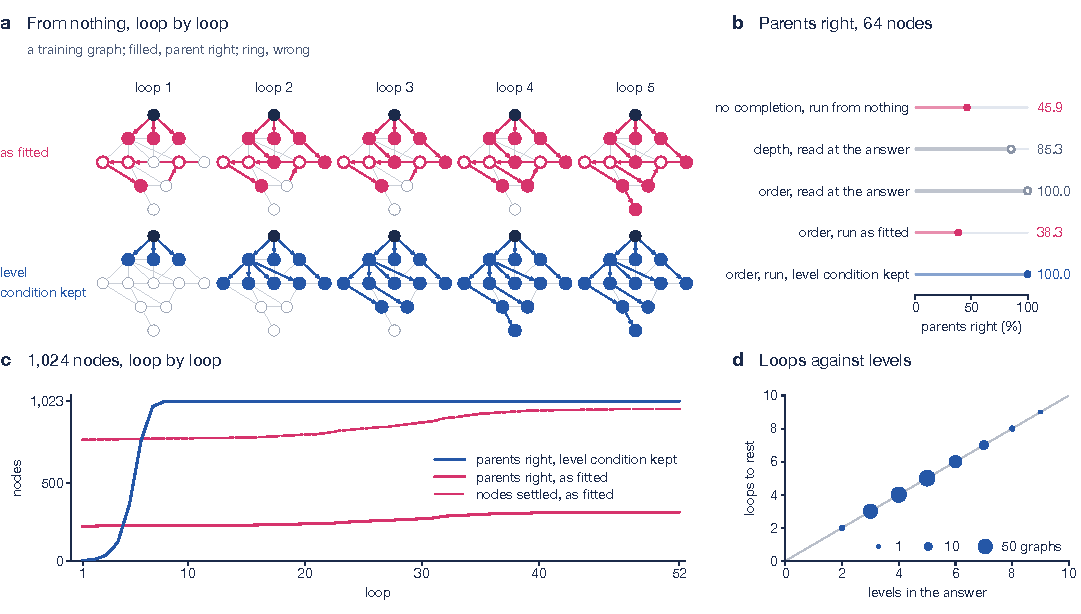
\includegraphics[width=\linewidth]{figures/fig2.pdf}
\caption[]{\figlabel{Fig. \thefigure}{A check is not yet a procedure.} Breadth-first search with queue-order parents (the textbook
labelling), as in Fig.~\ref{fig:idea}. Cobalt: the check run with the level condition kept; rose: the check
as fitted, and the fit with no completion; grey: checks read at the completed answer, not runs. \textbf{a}, The training
graph of Fig.~\ref{fig:idea}a run from nothing, loop by loop. A node is filled once it has a parent and the parent is right, a ring
if the parent is wrong, white while unsettled; arrows are the parents named so far. As fitted, the check names parents
for nodes two and three steps from the source in its first loop, before anything below them is placed, and three of
them are wrong. With the level condition kept it settles one distance per loop, all right. \textbf{b}, Parents right on
100 test graphs of 64 nodes (6,300 parents): with no completion, the fit run from nothing gets 45.9\%; with depth as the
completion, the check read at the answer gets 85.3\% (every parent it names is a valid shortest-path parent, but depth
does not hold the order of discovery that breaks the label's ties); with the order of discovery it gets 100\% read at
the answer, 38.3\% run from ``not yet'' as fitted, and 100\% run with the level condition kept (also at 256 and 1,024
nodes). \textbf{c}, The 1,024-node graph of Fig.~\ref{fig:idea}d,e: parents right after each loop, and the nodes the as-fitted run has
settled. Kept, every parent is right by loop 9; as fitted, 776 nodes are settled in loop 1 and
312 parents are right when the run stops at loop 52. \textbf{d}, Loops to rest against the number of levels in the answer (the distance of
the farthest node) on all 220 test graphs of 16, 64 and 256 nodes and the three of 1,024 (disc area: number of graphs, key at right):
the kept run stops after exactly as many loops as there are levels, as Proposition~2 bounds. Schematic: the node
positions in a (rows: distance from the source).}
\label{fig:theory}
\end{figure}

\section{Results}\label{sec:results}

\subsection{CRAM's benchmarks}\label{sec:cram}

We use CRAM's data, splits, test sets and operation count\cite{hoover2026classical}. On a grid, the check may use the
relations that cell coordinates express: same row, same column, same block for a block size $b$, the diagonals, and
conjunctions of two of these. The fit picks among them. This vocabulary is what lets one fitted rule serve every size;
CRAM instead learns a free table for each of the 3,240 pairs of cells of a Sudoku board.

\textbf{Sudoku.} On each of CRAM's three training splits of 1,000 solved boards, the fit
keeps exactly the 9 pair types that make up ``same row'', ``same column'' and ``same box'', and nothing
else. It takes 15 to 22 milliseconds on one CPU core. The rule solves all
412,786 test puzzles and never stops at a wrong board (Table~\ref{tab:cram}). It uses $5.6\times10^{4}$
operations a puzzle under CRAM's convention, 36,000 times fewer than CRAM, and $8.1\times10^{5}$ with
every comparison counted. The cold stage alone solves 13.9\% of the puzzles; a depth-first search
finishes the rest after a median of 45 choices. The same rule, unchanged, solves
1,000 of 1,000 puzzles of $4\times4$, all by the cold stage, 1,000 of 1,000 of
$16\times16$, and 100 of 100 of $25\times25$, with no wrong answer (Fig.~\ref{fig:puzzles}).
CRAM fits one model per board size.

\begin{table}[tbp]\centering\small
\caption{\figlabel{Table 1}{CRAM's benchmarks.} Operations a puzzle follow CRAM's convention, under which comparisons
are free; in brackets, every comparison counted as well. The rows for CRAM, its hand-set energy and TRMP, the most
accurate looped model, are from CRAM's Table~2 and Appendix~F\cite{hoover2026classical}. Our fit times are on one CPU
core, CRAM's on one H200 GPU. Ours on Sudoku-Extreme: each of three fits.}\label{tab:cram}
\begin{tabular}{llrrr}\toprule
Benchmark & Model & Solved & Operations a puzzle & Fit \\\midrule
Sudoku-Extreme (412,786) & TRMP, looped & 99.87\% & $4.6\times10^{12}$ & 9.0 h \\
 & CRAM & 99.996\% & $2.0\times10^{9}$ & 42 ms \\
 & CRAM, one weight set by hand & 100\% & $1.1\times10^{8}$ & none \\
 & \textbf{ours} & \textbf{100\%} & $5.6\times10^{4}$ ($8.1\times10^{5}$) & 15--22 ms \\\midrule
Maze-Unique (1,000) & CRAM & 100\% & $8.4\times10^{5}$ & 132 ms \\
 & \textbf{ours} & \textbf{100\%} & $1.6\times10^{4}$ ($6.6\times10^{4}$) & 24 ms \\\midrule
Maze-Hard (1,000) & CRAM, hand-built distance layer & 99.9\% & $1.4\times10^{7}$ & under 30 s \\
 & \textbf{ours}, the run's own clock & \textbf{100\%} & $2.0\times10^{3}$ ($6.2\times10^{3}$) & 33 ms \\\bottomrule
\end{tabular}
\end{table}

\textbf{Mazes.} On Maze-Unique the fitted rule says that an open cell on the path has exactly two path neighbours, and
the start and the goal one; the cold stage alone solves all 1,000 test mazes, and it is dead-end filling,
which we did not write in. The same rule is right on all 600 tree mazes of 29, 59 and 119 cells a side whose
dead ends reach the board's edge, on which CRAM's released model is right on none (Section~\ref{sec:cramweights}). On
Maze-Hard, which has loops and labels one particular shortest path, we replace CRAM's hand-built distance layer by the
cold run's own clock: the loop at which a cell is first reached from the goal, a register that every looped cold block
has. The fitted rule is to step to a neighbour reached one loop earlier and, among several, to prefer down, then left,
right and up. That order is the benchmark's own tie-break, learned from the labels, not set by us. The rule is right on
all 1,000 test mazes, including the one that CRAM's model misses on every seed. It is also right on all
136 mazes of rooms and corridors that we built to probe CRAM's model (Section~\ref{sec:cramweights}), and on
300 of 300 mazes with loops of 31, 61 and 121 cells a side.

\textbf{N-Queens and colouring.} Fitted on the 92 solutions of the $8\times8$ board, the same procedure keeps the costs
for two queens on a row, a column or a diagonal. It completes 100 of 100 boards at $80\times80$ and
at $100\times100$, whether nine queens are missing, seven eighths of them or all of them. Fitted on planted
3-colourable graphs of 10 vertices, it keeps only ``the same colour across an edge'' and colours
100, 100 and 100 of 100 graphs of 100 vertices at average degrees
3, 4.5 and 6. These instances are ours, not CRAM's test sets.

\subsection{CLRS-30}\label{sec:clrs}

We fit each task on 100 inputs of the official training split, with no hints: 20 at each of the
sizes 4, 7, 11, 13 and 16, or, for the string matchers, at the library's one training length of 20 items. We score with
the library's scorer on the official test at 64 nodes. For larger sizes we use our own generator, which reproduces every
official test split we use bit for bit and agrees with all 2,762,928 labels stored in the library's files for
22 of the tasks; held-out inputs are drawn at seeds never used before.

\textbf{All thirty tasks are exact} on the official test and on every held-out set (Table~\ref{tab:clrs}): the official
validation split, fresh inputs at 64 nodes, and fresh graphs of 256 and 1,024 nodes, dense as the library
draws them and sparse with about four neighbours a node; arrays and strings go to 4,096 and
5,120 items. That is 129 held-out sets with no miss (Fig.~\ref{fig:clrs}).

Fifteen tasks are learned from comparisons, counts and the completion, thirteen of them with nothing
supplied at all: the four sorts, minimum, binary search, quickselect, activity selection, breadth-first search, the
minimum spanning trees of Kruskal and Prim, and the naive and Knuth--Morris--Pratt string matchers. Task scheduling reads
its deadlines in the units of positions, and longest common subsequence reads each cell's count one cell up and one cell
left. Their completions are the depth along the answer's pointer, the bottleneck closure of the input's weights and the
closure of agreeing runs of text. With distinct weights, which the library's continuous weights make almost sure, an edge
is in the minimum spanning tree exactly when its weight equals the bottleneck (the cycle property), and the fit finds that
test; Prim's rule then walks that tree from the root, one level per loop. Each rule is fitted in 18 ms to
4.1 s on one laptop core and runs cold in at most 203 loops at 64 nodes. The other fifteen
read one quantity we supply, named in the table: the sum of a distance and an edge weight for the shortest-path
algorithms, the orientation of three points for the geometry tasks, the cost of a split for the two dynamic programmes,
prefix sums for the maximum subarray, closures of the graph with a node or an edge removed for articulation points and
bridges, and, for the depth-first family, an ``open'' bit with a check fitted at every prefix of the answer's own
preorder, the one family that sees more than the finished answer.

The fitted rules are conjunctions of one to seven conditions, chosen by the fit from thousands of candidates, and they
read like the library's own definitions (Box~1). Task scheduling's count rule is exactly the library's greedy, which
accepts a task while fewer tasks are chosen than its deadline, and the matchers return the first match, as the library
labels it. For binary search and segments intersect, a learned score also decides among the candidates that pass. What
the check learns is what the answer is, so tasks that share an answer share a rule: the four sorts learn one, the two
matchers one, the two hulls one, and Bellman--Ford and Dijkstra one, and the cold run is the procedure that
computes it, one loop for the sorts and Bellman--Ford's relaxation for the paths (Proposition~\ref{prop:bf}). With 10
training inputs instead of 100, 17 of the 19 tasks we tried stay exact, fitted in
6 to 521 milliseconds. Against the looped blocks of our earlier paper, which trained for about
an hour on a GPU per task\cite{mohsenvand2026zero}, the gain is in cost and in reach, and on longest common subsequence,
both string matchers, activity selection, task scheduling and Prim, in exactness.

\begin{figure}[tbp]\small
\fbox{\parbox{0.97\linewidth}{\textbf{Box 1 $|$ Six rules as fitted}, written out from the fitted tables; $k$ ranges over
third items ($k\neq u,v$), $u\to v$ is the ordered pair, and $\notyet$ marks an item the partial answer has not
reached.\\[0.4em]
\textbf{Insertion sort}, $u$ comes just before $v$: \ $\mathrm{key}_u<\mathrm{key}_v$, and no $k$ with
$\mathrm{key}_u<\mathrm{key}_k<\mathrm{key}_v$.\\[0.25em]
\textbf{Quickselect}, $i$ is the median: \ not $\#\{k:\mathrm{key}_k<\mathrm{key}_i\} < \#\{k:\mathrm{key}_k>\mathrm{key}_i\}$,
and not $\#\{k:\mathrm{key}_k\geq\mathrm{key}_i\} < \#\{k:\mathrm{key}_k<\mathrm{key}_i\}$.\\[0.25em]
\textbf{Kruskal}, $(u,v)$ is in the tree: \ an edge between $u$ and $v$ whose weight equals the bottleneck between $u$ and $v$, the
least possible largest weight on a path joining them (the cycle property).\\[0.25em]
\textbf{Activity selection}, $i$ is chosen: \ no chosen $k$ that finishes before $i$ finishes and after $i$ starts, the
answer read only downward along finish times.\\[0.25em]
\textbf{Breadth-first search}, $u$ is the parent of $v$: \ $\mathrm{depth}_u<\mathrm{depth}_v$, an edge $u\to v$, $u$
reached, $v$ not the source, and no $k$ with an edge $k\to v$, $\mathrm{depth}_k<\mathrm{depth}_v$ and a lower number
than $u$.\\[0.25em]
\textbf{Dijkstra}, with the sum supplied by hand (a ceiling): \ $\mathrm{dist}_u<\mathrm{dist}_v$, an edge $u\to v$, $u$
reached, $v$ not the source, and no $k$ with $\mathrm{dist}_k<\mathrm{dist}_v$ and
$\mathrm{dist}_k+w_{kv}<\mathrm{dist}_u+w_{uv}$.\\[0.4em]
Each rule is a conjunction of the pair's own comparisons and at most one witness test or two count comparisons, the
reads of the cold layer. The fit was told none of these conditions. The comparisons $\mathrm{depth}_u<\mathrm{depth}_v$
and $\mathrm{dist}_u<\mathrm{dist}_v$ are the level condition, which a finished answer cannot contradict. Read cold from $\notyet$, the
breadth-first rule places the nodes at distance $t$ from the source at loop $t$. All thirty rules are in Supplementary
Note~2.}}
\end{figure}

\begin{table}[tbp]\centering\scriptsize
\caption{\figlabel{Table 2}{All thirty CLRS-30 tasks fitted at the answer and run cold,} grouped by what we supply by
hand. Supplied: the quantity given by hand; results that rely on one are ceilings for the fitted check. Fit: wall clock on one laptop core, from loading the training inputs to the fitted rule; strong components reuse
the depth-first check, with no fit of their own, so their time is the depth-first fit. Loops: the most the cold run took
on any test input. Official 64: the library's score on the
official test. Exact to: the largest held-out size, in nodes or items, at which every held-out input was exact, with the
code frozen. Ours, looped: the better of the general and the cold looped blocks of our earlier paper; FloydNet: its
reported score\cite{yu2026floydnet}; both from Supplementary Table~4 of ref.~\cite{mohsenvand2026zero}. The averages mix
ceilings with the method and are not a like-for-like comparison.}\label{tab:clrs}
\setlength{\tabcolsep}{4.5pt}
\begin{tabular}{llrrrrrr}\toprule
Task & Supplied & Fit & Loops & Official 64 & Exact to & Ours, looped & FloydNet \\\midrule
\multicolumn{8}{l}{\textit{Comparisons and counts}} \\
Insertion sort & -- & 36 ms & 1 & 100.00 & 4,096 & 100.00 & 100.00 \\
Bubble sort & -- & 35 ms & 1 & 100.00 & 4,096 & 100.00 & 100.00 \\
Heapsort & -- & 34 ms & 1 & 100.00 & 4,096 & 100.00 & 100.00 \\
Quicksort & -- & 34 ms & 1 & 100.00 & 4,096 & 100.00 & 100.00 \\
Minimum & -- & 18 ms & 1 & 100.00 & 4,096 & 100.00 & 100.00 \\
Binary search & -- & 216 ms & 1 & 100.00 & 4,096 & 100.00 & 94.47 \\
Quickselect & -- & 18 ms & 1 & 100.00 & 4,096 & 100.00 & 80.33 \\
Activity selection & -- & 351 ms & 38 & 100.00 & 4,096 & 99.94 & 95.30 \\
Task scheduling & deadline $\div n$ & 479 ms & 8 & 100.00 & 4,096 & 99.86 & 91.05 \\
Breadth-first search & -- & 491 ms & 10 & 100.00 & 1,024 & 100.00 & 100.00 \\
Kruskal & -- & 94 ms & 1 & 100.00 & 1,024 & 100.00 & 99.63 \\
Prim & -- & 4.1 s & 87 & 100.00 & 1,024 & 99.98 & 99.67 \\
LCS length & index shift & 86 ms & 203 & 100.00 & 1,024 & 95.66 & 95.70 \\
Naive string matcher & -- & 212 ms & 3 & 100.00 & 5,120 & 99.07 & 100.00 \\
KMP matcher & -- & 207 ms & 3 & 100.00 & 5,120 & 99.15 & 99.43 \\
\addlinespace[2pt]
\multicolumn{8}{l}{\textit{One arithmetic primitive supplied}} \\
Bellman--Ford & sum & 3.9 s & 13 & 100.00 & 1,024 & 100.00 & 100.00 \\
Dijkstra & sum & 4.1 s & 13 & 100.00 & 1,024 & 100.00 & 97.67 \\
DAG shortest paths & sum & 4.2 s & 9 & 100.00 & 1,024 & 100.00 & 100.00 \\
Floyd--Warshall & sum & 43.3 s & 8 & 100.00 & 256 & 100.00 & 96.20 \\
Graham scan & orientation & 42 ms & 1 & 100.00 & 1,024 & 99.80 & 99.63 \\
Jarvis march & orientation & 42 ms & 1 & 100.00 & 1,024 & 99.92 & 99.50 \\
Segments intersect & orientation & 45 ms & 1 & 100.00 & fixed size & 99.33 & 99.90 \\
Matrix chain order & products, sums & 61 ms & 20 & 100.00 & 128 & 99.80 & 91.50 \\
Optimal BST & sums & 78 ms & 8 & 100.00 & 128 & 82.71 & 82.87 \\
\addlinespace[2pt]
\multicolumn{8}{l}{\textit{Algorithmic structure supplied}} \\
Maximum subarray & prefix sums & 458 ms & 1 & 100.00 & 4,096 & 87.86 & 86.20 \\
Articulation points & deletion closure & 23 ms & 1 & 100.00 & 1,024 & 100.00 & 100.00 \\
Bridges & deletion closure & 26 ms & 1 & 100.00 & 256 & 100.00 & 100.00 \\
Depth-first search & ``open'' & 47.5 s & 257 & 100.00 & 256 & 100.00 & 100.00 \\
Topological sort & ``open'', finish order & 47.6 s & 257 & 100.00 & 256 & 100.00 & 100.00 \\
Strong components & two passes & 47.5 s & 257 & 100.00 & 256 & 90.61 & 90.07 \\
\midrule
Average (30 tasks) & & & & 100.00 & & 98.46 & 96.64 \\
\bottomrule\end{tabular}
\end{table}

\textbf{One check for several algorithms.} The fitted check can be shared across tasks, as the looped block of our
earlier paper was. One check, told nothing about which task it serves, fitted jointly on breadth-first search, Prim,
Bellman--Ford, Dijkstra and shortest paths in an acyclic graph in 40~s, is exact on all five, on the
official test and on fresh graphs of 1,024 nodes (Table~\ref{tab:shared}). One check serves the four sorts, fitted in
0.6~s, and one the five selection tasks (activity selection, task scheduling, both convex hulls and
articulation points), with or without a bit that names the task. Each task still reads its own completion and supplied
quantity; registers are matched by name across the pooled tasks, so a breadth-first state has no distance and every
comparison on one is false. The graph check is a conjunction of five conditions with the learned score deciding among the
candidates that pass (Supplementary Note~2). Sharing has a limit: one check for all nine pointer tasks keeps the sorts and the shortest paths exact but
falls to 32\% on breadth-first search and 36\% on Prim, with or without the task bit.
A single conjunction keeps only the conditions that hold for every pooled task, and with no disjunction a task bit
cannot switch a condition on for one task alone.

\begin{table}[tbp]\centering\scriptsize
\caption{\figlabel{Table 3}{One fitted check for several CLRS-30 tasks.} Each row is one check fitted jointly on the
training answers of all its tasks. Task named: whether a bit naming the task is among the inputs. Fit: wall clock on one
laptop core. Scores: the library's scorer on the official test and on fresh inputs of 1,024 nodes or items, per task.}
\label{tab:shared}
\begin{tabular}{lrlrp{0.2\linewidth}p{0.2\linewidth}}\toprule
One check for & Tasks & Task named & Fit & Official 64 (\%) & Fresh 1,024 (\%) \\\midrule
The four sorts & 4 & no & 0.6 s & all 100 & all 100 \\
Three shortest-path algorithms & 3 & no & 26.5 s & all 100 & all 100 \\
Five graph algorithms & 5 & no & 39.7 s & all 100 & all 100 \\
Five selection tasks & 5 & no & 4.2 s & all 100 & all 100 \\
Five selection tasks & 5 & yes & 3.8 s & all 100 & all 100 \\
Nine pointer tasks & 9 & no & 42.1 s & breadth-first search 31.6; Prim 35.9; others 100 & breadth-first search 24.9; Prim 3.1; others 100 \\
Nine pointer tasks & 9 & yes & 42.1 s & breadth-first search 31.6; Prim 35.9; others 100 & breadth-first search 24.9; Prim 3.1; others 100 \\
\bottomrule\end{tabular}
\end{table}

\subsection{Proofs at every size}\label{sec:proofs}

The fitted rules are small tables in which no size appears, so their correctness at every size reduces to finite
checks, which we ran by script (Supplementary Note~1 gives the arguments in full).

\emph{Sudoku.} A pair of cells has one of a fixed set of types, set by which coordinate relations agree, and the types
that a board realises do not change with the block size $b$ beyond $b=3$. A finite check confirms that the kept types
are exactly the row, column and box pairs at every $b$ from 2 to 8, on all three fits. Every
kept cost is at least 1.38, no cost is negative, and the stopping threshold is 0.001, so a board
passes the check exactly when no row, column or box holds a value twice. A unit of $n$ cells with $n$ values then holds
each value once: the stop is sound at every size. Each removal of the cold stage follows from a count condition that
holds on every valid board, so the cold stage never removes a value of any solution, and with the complete search every
puzzle that has a solution is solved given enough moves.

\emph{Mazes.} On any tree maze the true path meets every kept range, so no removal is ever wrong. From the all-open
start, the cold stage removes cells with fewer than two possible path neighbours until what is left is a subtree whose
only leaves are the start and the goal, which is the path. No size and no edge term enter. A brute-force check over all
108,084 spanning-tree mazes of the smallest lattices agrees. On Maze-Hard the clock is exactly the distance to
the goal, and the fitted rule takes the neighbour one step nearer and breaks ties by the label's own order, so it
returns the label on every maze of any size.

\emph{CLRS-30.} Proposition~\ref{prop:finite} applies to the sorts, minimum, Kruskal and breadth-first search, whose
rules use only own comparisons and witness tests. For the four sorts we checked every order of distinct keys, as the
library draws them, on up to 5 items (3,447 pairs each), and for minimum up to
4. Kruskal's and breadth-first search's rules read a completion, the bottleneck or the depth, so their
certificates work on the completed input, with the register given and constrained only by local axioms (Supplementary
Note~1). For Kruskal we checked every value the axioms allow against the cycle property, with distinct weights; for
breadth-first search, all 274,688 pair cases on up to 4 items. These certify the check at
the answer at every size. That the cold run reaches the answer is Proposition~\ref{prop:bf} for the shortest-path tasks,
and the level-by-level argument of Supplementary Note~1 for breadth-first search, Prim and the greedy tasks.

\subsection{What CRAM's released weights show}\label{sec:cramweights}

The same reading applies to CRAM's own released models, and it explains their two failures. Everything here comes from
the authors' public checkpoints and code, run unchanged.

\emph{The hidden layer cools.} For Maze-Hard, CRAM gives each open cell a hidden value $\psi$, updated as
$\psi_i \leftarrow \log(4+m) - \log \sum_{j \sim i} e^{-\psi_j}$ plus a source at the goal, which the authors' code
calls a soft-min Bellman backup. One learned number, the mass $m$, sets its temperature: a step of distance costs
$\log(4+m)$, so the temperature, in steps, is $1/\log(4+m)$. This is a walk distance, the family that runs from
random-walk distances at high temperature to the shortest-path distance at zero\cite{chebotarev2012walk,kivimaki2014developments}.
Over training the cost of a step rises from 5.4 to 19.7 on seed 0, and to between
19.7 and 19.8 on all three seeds, with the mass at $3.7\times10^{8}$ and still rising at the
last step. Gradient descent is driving the layer towards a hard minimum, the read our cold layer takes, and a
temperature can only approach zero.

\emph{Where it is still warm, the tie count leaks in.} At any temperature above zero, the hidden value of a cell is
approximately its distance to the goal times the cost of a step, minus the logarithm of the number of shortest routes
from the cell. The walk-distance literature knows the second term as one that vanishes in the
limit\cite{francoisse2017bag}. Read cold, the distance and the tie count are separate numbers, the best witness and the
number tied with it in our earlier paper. Read warm, they are added, and a cell with many shortest routes looks nearer
than it is. The model's pointer adds learned scores for the four directions, 9.35 for down, 1.69
for left, $-$1.93 for right and $-$9.37 for up, exactly the benchmark's tie-break order, so a large
enough room of equally short routes outweighs the gap between two directions. With $\psi$ approximately $c$ times the
distance minus the log of the number of shortest routes, $c$ the cost of a step, the pointer leaves a corridor for a
room of equal length once the log of the room's route count exceeds the gap between their two direction scores. For the
corridor down and the room to the left that gap is 7.66: a room of $7\times7$ cells has 924
corner-to-corner routes ($\ln = 6.83$), and one of $8\times8$ has 3,432 ($\ln =
8.14$). Settling the released hidden layer on each maze and reading its pointer gives the same switch.
We built 136 mazes of rooms
and corridors to test it and ran the full released models. On every seed,
20 of the mazes are not given the label's path, from rooms of 8 by
8 cells, and 5 to 6 of those are given
a path two steps longer than the shortest (and one, on one seed, a set of cells that is not a path). Our rule, which
keeps the clock and the direction apart, is right on all of them.

\emph{The maze rule fails at the edge.} CRAM's Maze-Unique model sees a cell and its eight neighbours. Of the
256 patterns a cell inside the board can see, the released weights follow the dead-end rule on all,
on every seed, which with a short induction proves the model exact inside the board at every size. On the board's edge
they break it on 12 of 32 patterns, and in a corner on 4 of
8. A wall next to a cell adds a cost for keeping it open, and beyond the edge there is no wall, so a
dead end that stops at the edge is never filled. CRAM's test set has no open cell on the edge. On our 600 tree
mazes with a ring of wall the released model solves 600 of 600 on every seed; on the same
mazes without the ring it solves none on any seed. The one Maze-Hard failure the authors report, a dead end of six
cells left open along the border of test maze 106, fits the same explanation.

\emph{CRAM's own stop can be proved sound.} The authors observe that their Sudoku search never stops at a wrong board.
Their models also hold 426 to 471 small negative costs on pairs of cells that share no unit, so
the observation does not follow at once. A short counting argument shows that a wrong board has at least two clashing
pairs. On each seed it therefore pays at least 0.97 to 0.99 in costs and can earn back
at most 0.67 to 0.76, so every wrong board lies at least 0.23
above zero, far above the threshold of 0.001. The stop is sound for every one of the $9^{81}$ boards.

\begin{figure}[tbp]
\centering
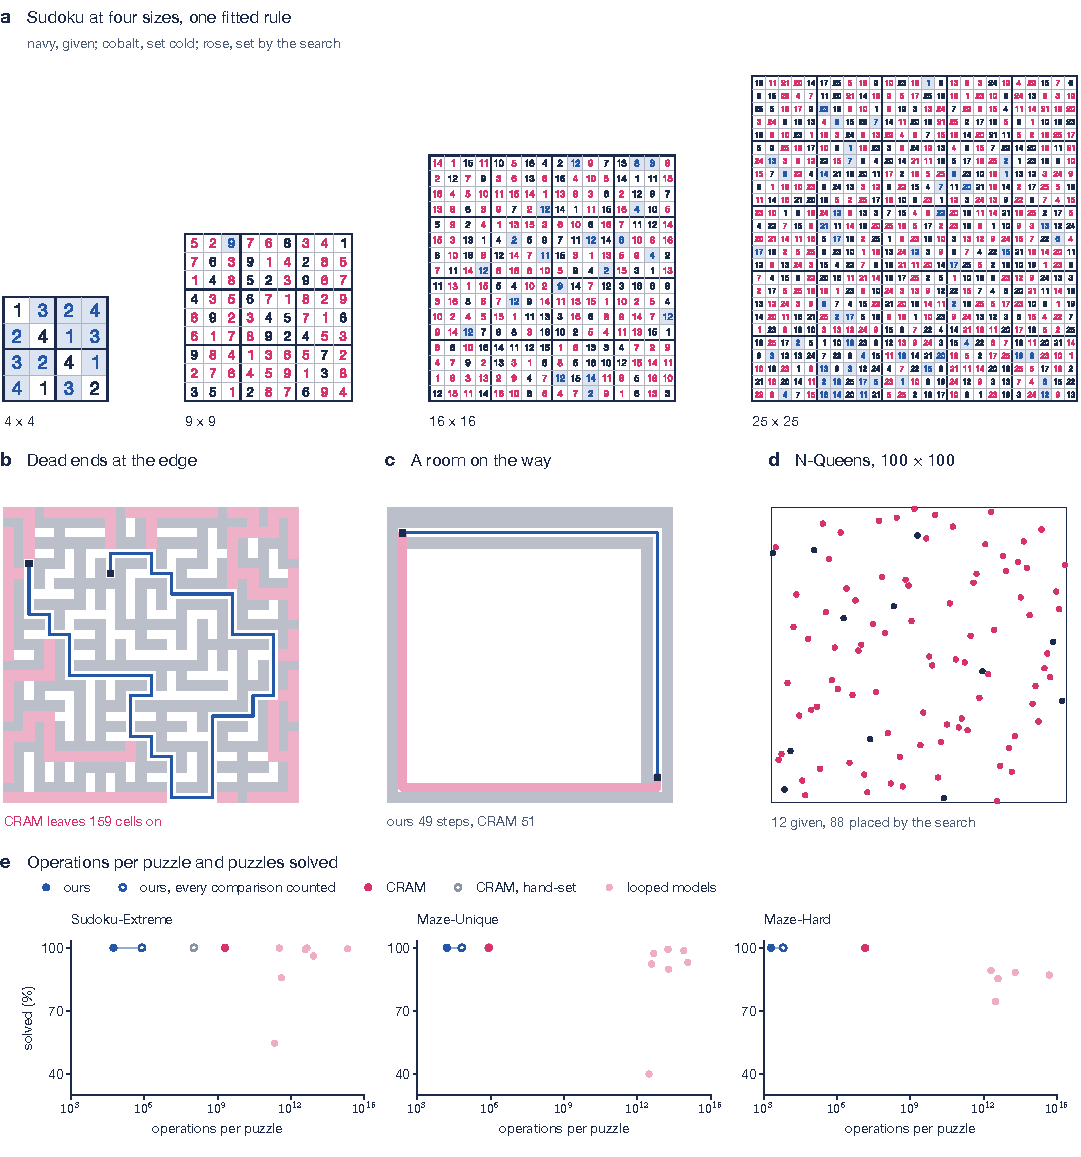
\includegraphics[width=0.92\linewidth]{figures/fig3.pdf}
\caption[]{\figlabel{Fig. \thefigure}{One fitted rule on CRAM's benchmarks.} Cobalt: our fitted check, run cold; rose: our search where the
cold stage forces nothing, and CRAM; pale rose: the looped models. \textbf{a}, The rule fitted in 22 ms on
1,000 solved 9\,$\times$\,9 boards, unchanged, on boards of four sizes: digits given (navy), set by
the cold stage before any search (cobalt, tinted cells), and set during the search (rose), whose stopping test is the
same check; one engine for every size (the cold stage with its deduction over pairs of units, and a restarted search). 4\,$\times$\,4: 11 of 11 blanks set cold. 9\,$\times$\,9: a Sudoku-Extreme test puzzle (the first that
needed at least the median number of search moves), 1 set cold and 55 by the search in 246 moves. 16\,$\times$\,16: 19
cold, 142 by the search. 25\,$\times$\,25: 51 cold, 293 by the search in 1,514 moves. The 4\,$\times$\,4,
16\,$\times$\,16 and 25\,$\times$\,25 puzzles are generated with one solution each. \textbf{b}, A tree maze of
29\,$\times$\,29 cells whose dead ends reach the board's edge (the first of the 200 at this size): the path, which our
rule returns, and in rose the 159 further cells that CRAM's released Maze-Unique model leaves on (its training mazes never
touch the edge); over all 600 such mazes ours is right on 600 and CRAM's on 0.
\textbf{c}, A room-and-corridor maze: ours returns the label's shortest path (cobalt, 49 steps); CRAM's released
Maze-Hard model returns a valid path two steps longer (rose band, 51 steps), the smallest room at which it leaves the
shortest path in this orientation. \textbf{d}, N-Queens on a 100\,$\times$\,100 board from 12 given queens (navy), with
the rule fitted on the 92 solutions of 8\,$\times$\,8: the cold stage forces none here and the search places the other
88 (rose) in 81 moves (a move is one choice; the cells the cold stage forces after it are not counted). \textbf{e}, Operations per puzzle against puzzles solved on CRAM's test sets (CRAM's convention,
comparisons free; open cobalt mark: every comparison counted too). Sudoku-Extreme: ours $5.6\times10^{4}$
($8.1\times10^{5}$) on all 412,786; CRAM $2.0\times10^{9}$ at 99.996\%; CRAM with hand-set
weights $1.1\times10^{8}$; seven looped models from CRAM's Table 2. Maze-Unique: ours $1.6\times10^{4}$, CRAM
$8.4\times10^{5}$. Maze-Hard: ours $2.0\times10^{3}$, CRAM with its hand-built distance layer $1.4\times10^{7}$ at
99.9\%, and five looped models from CRAM's Table 8. Released models: seed 0. Schematic: none; every cell and
mark is data (the operation axis is logarithmic).}
\label{fig:puzzles}
\end{figure}

\begin{figure}[tbp]
\centering
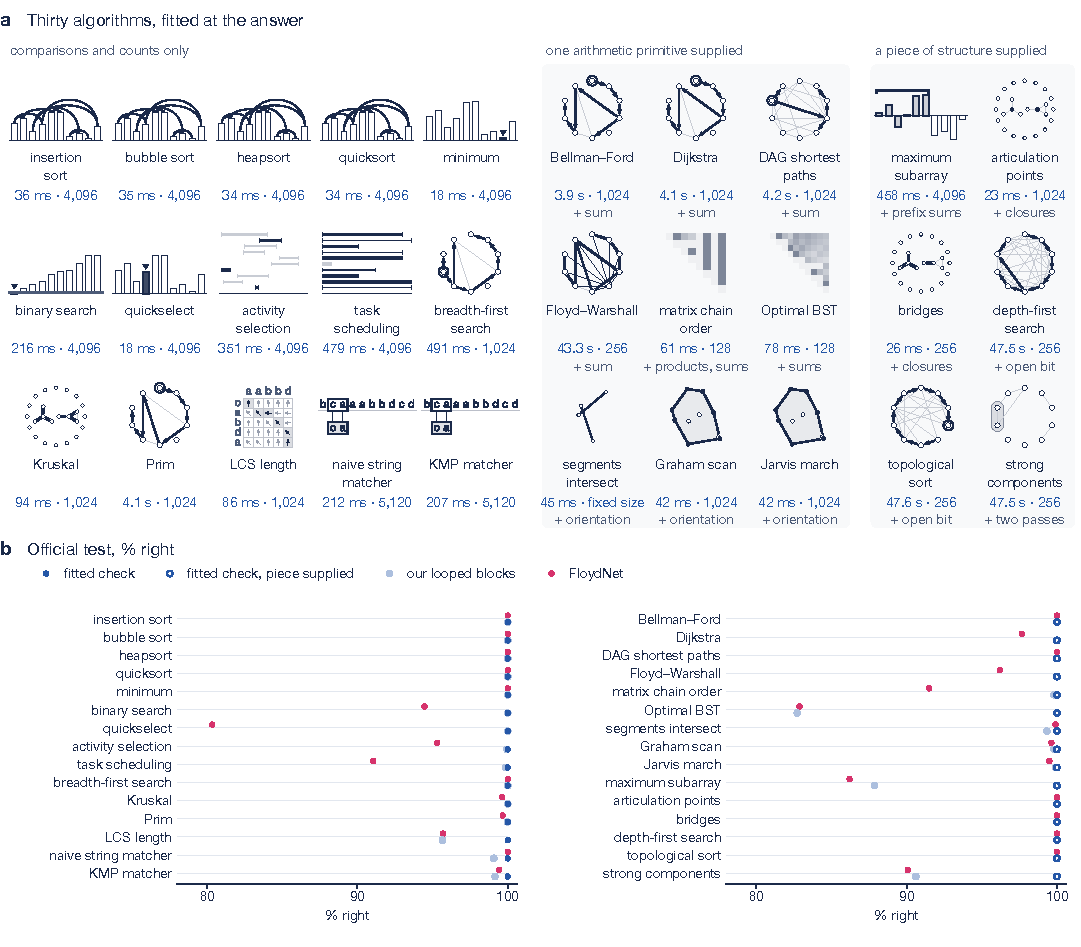
\includegraphics[width=\linewidth]{figures/fig4.pdf}
\caption[]{\figlabel{Fig. \thefigure}{CLRS-30, fitted at the answer.} Cobalt: our fitted checks; pale cobalt: our looped blocks of the
earlier paper; rose: FloydNet. \textbf{a}, The thirty tasks, in three groups by what we supply by hand. Left,
15 tasks learned with comparisons, counts and the completion of the answer (task scheduling's deadlines in units
of positions and LCS's one-cell index shift set by hand, marked + units and + shift). On a pale band:
9 tasks given one arithmetic primitive and 6 given a piece of algorithmic structure (named
under each). Each glyph is a small input of the benchmark's own generator with its true answer drawn in navy over the
input in grey, in the layouts of our earlier paper's Fig.~5a; every fitted check returns the true answer on every
official and held-out test input. Under each task: the time to fit its rule on one laptop core (topological
sort and strong components reuse the depth-first check), and the largest held-out
size at which every input was exact (segments intersect always has four points). \textbf{b}, Percent right on the
official 64-node test: our fitted check is exact on all thirty (filled: comparisons and counts; open: a piece supplied), against the
better of our general and cold looped blocks and FloydNet's reported score, both from our earlier paper's
Supplementary Table~4. Schematic: the glyphs' layouts (node order around each ring, the arcs of the sorting tiles, the
tints of the split tables, the placement of the 24-node graph).}
\label{fig:clrs}
\end{figure}

\begin{figure}[tbp]
\centering
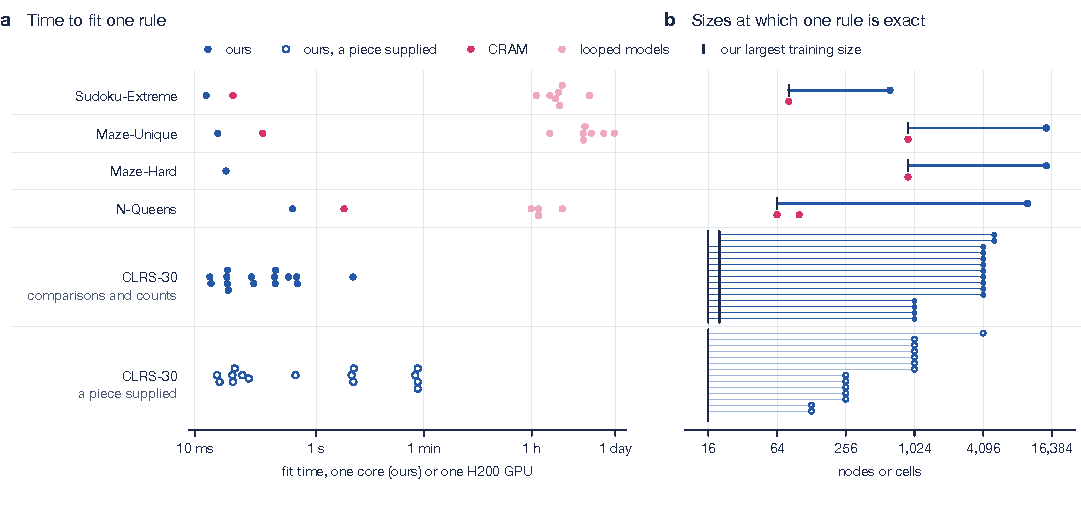
\includegraphics[width=\linewidth]{figures/fig5.pdf}
\caption[]{\figlabel{Fig. \thefigure}{Fitted in milliseconds, exact far beyond training.} Cobalt: ours (open: CLRS-30 tasks given a piece by
hand); rose: CRAM; pale rose: the looped models. Both axes are logarithmic. \textbf{a}, The time to fit one
rule: ours on one laptop core, from the training answers to the fitted rule, completions and candidate conditions
included (CRAM's benchmarks: the median of warm fits; CLRS-30: the best of three), CRAM and the looped models on one H200 GPU as CRAM reports them (its Tables~2 and~3; no fit times
are reported for Maze-Hard, and N-Queens is CRAM's 8\,$\times$\,8 model). Within a row, marks that would overlap are
stacked; only their horizontal position is data. \textbf{b}, The sizes, in nodes or cells, at which one fitted rule is
exact: a line from our largest training size (tick) to the largest held-out size at which every test was exact (dot).
CRAM fits and tests each model at one size (rose); the looped models are trained and tested at the same sizes. Sudoku:
fitted at 9\,$\times$\,9, exact at 4\,$\times$\,4, 16\,$\times$\,16 and 25\,$\times$\,25 (625 cells). Mazes: exact up to 121
cells a side. N-Queens: fitted on 8\,$\times$\,8, exact at 100\,$\times$\,100. CLRS-30: one line per task, trained at
16 items (the string matchers at 20); segments intersect, at a fixed size of four points, is not drawn.}
\label{fig:cost}
\end{figure}

\section{Related work}\label{sec:related}

Much of the skeleton of this setting is classical. Markov logic networks tie rules by role across all their groundings, fit them by pseudolikelihood, and solve them by
local search that stops when every hard clause holds\cite{richardson2006markov}. Their authors also noted that pseudolikelihood can do badly when long chains of
inference are needed\cite{lowd2007efficient}. One conditional model per relation, with counts over related objects as
features, is a relational dependency network\cite{neville2007relational}, and counting the third objects that pass a test
on both legs is one of the complex aggregates of relational decision trees\cite{vens2006refining}. Asking that each
solved example be a model of the learned rules is learning from interpretations\cite{deraedt1994first}. Programs with
recursion are learned exactly from examples by inductive logic programming: ILASP learns answer set programs whose
examples must be answer sets\cite{law2014inductive}; Popper searches for recursive programs\cite{cropper2021learning};
differentiable forward chaining learns rules by unrolling inference\cite{evans2018learning}. ``Derive what is forced,
then guess and check'' is how answer set solvers work, starting from the well-founded model\cite{vangelder1991well}.
Constraint acquisition learns count constraints from solutions, and COUNT-CP transfers them from $4\times4$ to $9\times9$
Sudoku\cite{kumar2022learning}. Every symbolic learner here searches the space of rules; we fit a fixed family of
conditions in one step.

On the neural side, CRAM is the immediate starting point\cite{hoover2026classical}, and energies for reasoning are an
active line\cite{du2022learning,chen2026energy}. Looped networks trained on small mazes and run on far larger ones go
back to Deep Thinking\cite{bansal2022end}. Recurrent and message-passing reasoners now transfer across sizes on
constraint problems\cite{toenshoff2023one,salvatori2026tiny}, and lattice deduction transformers, which project a
recurrent state onto a lattice at every step, solve all of Sudoku-Extreme\cite{davis2026lattice}. In algorithmic reasoning, hints supervise a network
on an algorithm's trace\cite{velickovic2022clrs}, and a no-hint mode trains on answers alone, through the
loop\cite{rodionov2023neural}. Discrete neural algorithmic reasoning proves its learned executions correct on any input
but trains on hints\cite{rodionov2025discrete}. Dual algorithmic reasoning adds an optimality certificate as extra
supervision\cite{numeroso2023dual}, and a sparsity regulariser lets a network trained on a few shortest-path instances
provably approximate Bellman--Ford at every size\cite{nerem2025graph}. Proof labelling schemes and locally checkable
proofs study, in distributed computing, which global properties have labels that a local verifier can
check\cite{korman2010proof,korman2007distributed,goos2016locally}.

Against this background, our contributions are four. The first is the cold pair read with comparisons of counts,
fitted at the answer with no search over programs: one greedy pass over a fixed family of conditions. The second is
the answer completed by closures and counts as the training target. It links the hints of algorithmic reasoning to the
labels of proof labelling schemes: a completion is a certificate computed from the answer instead of from the trace.
The third is the level condition. Keeping every condition that held on all positives is the most specific conjunction
of inductive logic programming, the least general generalisation and its bottom clause\cite{plotkin1970note,muggleton1995inverse};
what is new is to keep it because it carries Fages' level mapping, so that the answer the fitted check supports is the
least model it computes. The fourth is proofs at every size from a table fitted at the answer, without a trace. Discrete
neural algorithmic reasoning proves its executions correct on any input from hints\cite{rodionov2025discrete}, Nerem
et al.\ prove a regularised network approximates Bellman--Ford at every size\cite{nerem2025graph}, and our earlier paper
certified trained blocks by finite checks\cite{mohsenvand2026zero}; here the table comes from one fit at the answer.
\section{Discussion}\label{sec:discussion}

A fit at a solved example has always been cheap, and it has always learned a check. We have shown when that check is
the algorithm: when the answer is completed with the labels that let a local rule verify it, and when the condition that
orders the answer, invisible at the finished answer, is kept in the rule. Then the fit of a few milliseconds and the
procedure that runs at any size are the same object. Because that object is a small table with no size in it, its
correctness can be proved rather than measured. The cold layer of our earlier paper was built for this. Its reads,
whether a witness exists and how two counts compare, are the conditions that survive a change of size, and its zero
temperature keeps a tie count from leaking into a distance, as it does in CRAM's warm hidden layer.

\textbf{Limitations.} Fifteen CLRS-30 tasks read a primitive or a piece of structure we supply, from a sum to the open
nodes of a depth-first search, and two more a change of units or an index shift; they show what the check does with the
right quantity, not that it finds it. On grids, the coordinate vocabulary
is a prior that CRAM does not use, and the puzzle search is a classical depth-first search.

Two directions are open. One is to search for the completion itself: closures and counts form a small grammar, and a
completion that makes the training answers locally checkable is a target a search can recognise. The other is to put
the check where our earlier layer stands, beside a language model, where a fit of milliseconds could replace hours of
training through loops.
\section*{Methods}

\paragraph{Benchmarks and protocol.} CRAM's benchmarks are read from the files at the revisions CRAM pins
(Sudoku-Extreme, Maze-Hard and Maze-Unique), with CRAM's own split index; the Sudoku-Extreme test set rebuilt from the
official file matches the hash that CRAM records. Sudoku-Extreme follows CRAM's protocol: three fits, one on each of its
training splits of 1,000 boards, each scored once on all 412,786 test puzzles. A puzzle
counts as solved when the board returned equals the dataset's solution. Operations follow CRAM's convention (its
Appendix~C.2: additions count, comparisons and mask logic do not); we also report the count with every comparison
included, which is the fairer number for a search like ours. CLRS-30 inputs, answers and scores come from the
benchmark's library\cite{velickovic2022clrs}. Our generator reproduces the official test split of every task, and
relabels every stored training, validation and test split with no wrong label. Held-out inputs are drawn at seed
$9000 + n$, never used during development, with the official test's numbers of inputs at 64 nodes, and are scored with
the code frozen.

\paragraph{Completion.} The completions of CLRS-30 are computed from the final answer or from an input relation, by
closure and counting, never from a step of the algorithm. Depth is the number of ancestors along the answer's pointer
(Eq.~\ref{eq:completion}); its weighted form, the sum of edge weights along the pointer, is used only by the four
shortest-path tasks. Both are computed by pointer doubling from the source, so a node the pointer does not join to
the source keeps $\notyet$. The bottleneck closure of the weights is the closure of the edge weights in the (min, max) semiring. The run
closure of the string matchers marks a pair (text position $t$, pattern position $p$) when the two letters agree and
either $p$ is the pattern's last letter or $(t+1, p+1)$ is marked. For longest common subsequence the completion is the
number of match arrows along the answer's arrows from each cell, and each cell reads that count one cell up and one cell
to the left; this shift is supplied by hand. On puzzles nothing is completed: Sudoku shows every cell, and the maze
clock is the cold reach run's loop of first arrival.

\paragraph{Conditions.} For every task the family $\Phi$ is built from the input types alone, as in
Section~\ref{sec:setting}. Item registers are compared with $<$, $\leq$, $=$, $\geq$ and $>$; for a number $a$, $a<\notyet$,
$a\leq\notyet$, $\notyet>a$ and $\notyet\geq a$ hold, and every other comparison with $\notyet$, including $\notyet$
against $\notyet$, is false. Pair numbers, such as the edge weight $w$, the bottleneck $B$ and, for the shortest-path
tasks, the supplied sum $S(u,v) = \mathrm{dist}_u + w(u,v)$, are compared with $<$, $=$ and $>$: with each other on the
same pair; with an item register (Floyd--Warshall's self-loop weight); and through a third item, $\exists
k\notin\{u,v\}$ with a leg into $v$ and $N_1(k,v)$ against $N_2(u,v)$. Witness tests read $\exists k\notin\{u,v\}:
A(u,k)\wedge B(k,v)$; a leg is a test on the pair it joins (a relation, a register comparison or a pair-number
comparison), optionally a relation or pair-number comparison conjoined with a register comparison, optionally with a bit
of $k$. Count conditions, for item targets, compare $\#\{k : A(k,i)\}$ with $\#\{k : B(k,i)\}$ ($<$ or $=$, both orders)
for two legs. Any condition can enter a rule negated. Numbers never enter except through comparisons, and no condition
names a position or a size.

\paragraph{Fitting.} Each output (a pointer off the diagonal, a pointer to itself, an item mask, a pair mask) is fitted
on the rows of the completed training answers: every candidate pair or item, labelled by the answer. First, every own
condition that held on all training positives, and failed on at least $\max(10, 0.5\%)$ of the rows, is kept
(Eq.~\ref{eq:kept}). Second, conditions true on every positive are added greedily, each time the one that rejects the
most negatives still passing, until no training negative passes\cite{haussler1988quantifying}. Third, a logistic
regression with an $\ell_1$ penalty over all conditions scores the candidates; it only breaks ties between candidates
that pass, except for binary search and segments intersect, where no conjunction is exact on the training answers and
the score decides. Where an output feeds back into the check as item bits (the greedy tasks and the string matchers),
the answer is read only downward along one order, and the fit tries each register and direction and keeps the one
whose rule is exact at the training answers; this order is Fages' level mapping chosen by the data (finish time for
activity selection, weight for task scheduling, position for the matchers). A target's own completion value enters its register comparisons only as ``the other
item is below me''; pair numbers that contain it, such as $S$ on the legs of a node's own self-pointer rule, are not
filtered.

\paragraph{The cold run.} The run starts with no pointer, no selection and no arrow, and every register at $\notyet$.
Each loop recomputes the completion from the current partial answer by the same code as at the answer, and decides every
item from that one state. A pointer is written only where a candidate passes, the self-pointer by its own rule; among
several, the higher score wins, and a node with no passing candidate keeps no pointer, which at rest is written as a
self-pointer, the library's ``none''. Depth and distance count only from the source, so a provisional self-pointer
leaves a node at $\notyet$. Binary search returns the passing item with the highest score; segments intersect answers
yes when every item passes its rule. The run stops when a loop changes nothing, and every run we report came to rest.

\paragraph{Puzzles.} Cells carry coordinates, and a pair of cells is described only by which coordinate functions agree:
for a grid of side $n=b^2$, the row, the column, $\lfloor r/b\rfloor$, $\lfloor c/b\rfloor$, $r \bmod b$, $c \bmod b$,
$r-c$ and $r+c$. Because overlapping relations such as a row and its band predict a solved board equally well, the fit
is made on the disjoint pair types, the full pattern of agreements, with costs kept non-negative, and the kept relations
are read off the kept types. Values are compared only as the same or different. The pseudolikelihood fit with an
$\ell_1$ penalty takes two to four full-batch steps on the 1,000 training boards. For every kept
relation, the range of ``how many related cells hold value $v$'', given whether the cell holds $v$, is recorded over all
training answers; on mazes these counts run only over cells on the path, so that a missing neighbour beyond the board's
edge counts as nothing. The cold stage keeps a set of possible values for each cell, bounds each kept count from below
by the cells fixed to $v$ and from above by the cells that may still take $v$, removes a value when a range can no
longer be met, and repeats until nothing changes. On Sudoku it also reasons over pairs of overlapping units, a propagation
rule we wrote over two fitted count conditions, not fitted itself: if all the places of $v$ in a unit $A$ lie inside a
unit $B$ that allows $v$ at most once, then $v$ leaves the rest of $B$. The search picks the open cell with the fewest possible values, tries them in a random order, runs
the cold stage after each choice and undoes on a contradiction, restarting on the Luby schedule\cite{luby1993optimal}
with a base of 10,000 moves, within a budget of $10^{7}$ moves. A move is one value tried at one branch
point; cells the cold stage forces after it are not counted. The generated Sudoku boards permute the rows, columns,
bands, stacks and digits of a pattern solution, then blank cells in random order, keeping a blank only when an exhaustive
search proves the puzzle still has one solution: $4\times4$ and $16\times16$ boards are blanked until no further cell
can go, and $25\times25$ boards until 55\% of cells are blank. On Maze-Hard the reach run starts at the
goal, at loop 0, and each loop adds the open side neighbours of the cells reached in the loop before, so the clock is the
distance to the goal. On Maze-Hard the
path rule is fitted on the 114,064 consecutive steps of the training labels, over three kinds of feature: the
neighbour is open, its clock compared with the cell's, and the direction of the step. For N-Queens we fitted on the 92
solutions of $8\times8$ and tested on 100 random solutions each of $80\times80$ and $100\times100$, generated by
min-conflicts, completed from three starts: nine queens removed, $N - \lfloor N/8 \rfloor$ removed (88 of 100), and the
empty board. For colouring
we fitted on 1,000 planted 3-colourable graphs of 10 vertices (random colour classes, edge probability 0.5 across
classes) and tested on 100 planted graphs of 100 vertices at each expected average degree. The tree mazes without a ring
are the ringed mazes of 31, 61 and 121 cells a side with the outer ring of wall removed.

\paragraph{Supplied by hand.} Group one: deadlines divided by the number of tasks (task scheduling) and the one-cell
shift of longest common subsequence. Group two: the sum $S(u,v) = \mathrm{dist}_u + w(u,v)$ for Bellman--Ford, Dijkstra,
shortest paths in an acyclic graph and Floyd--Warshall, which we read as one single-source problem per source, with the
weight of a self-loop as an item number for its diagonal; the sign of the orientation of three points for Graham scan,
Jarvis march and segments intersect, with the read-out ``every point passes'' for the last; and, for matrix chain order
and optimal BST, the cost of splitting an interval at each point, on a cost table completed from the answer's
own table of splits by its recursion. Group three: for the maximum subarray, prefix sums, their running minimum and the
best sum ending at each item; for articulation points and bridges, the components of the graph with one node, or one
edge, removed; for depth-first search, the bit ``placed and with an out-neighbour not yet placed'' on each node, the check
fitted at every prefix of the answer's own preorder (48~s, the one slow fit) and the run placing one
node per loop, which a P-complete problem such as lexicographic depth-first search\cite{anderson1987parallelism} leads
us to expect; for
topological sort, the finish order read from the cold depth-first search; and for strongly connected components, two
passes of the same check, the second on the reversed graph in order of decreasing finish time, and a closure that names
each tree by its root.

\paragraph{Proofs.} The finite checks are scripts that rebuild each fitted rule from its saved table and evaluate it with
the code that ran it: on every Sudoku pair type at block sizes 2 to 8; on every spanning-tree maze of the $2\times2$,
$2\times3$ and $3\times3$ room lattices, with and without a ring of wall, for every start and goal; and on every input
of the CLRS-30 certificates' sizes. The arguments are in Supplementary Note~1. None is yet in Lean.

\paragraph{CRAM's released models.} We read the authors' released checkpoints and ran their own code, unchanged, on CPU.
The runs first reproduce the recorded scores (99.9\% of Maze-Hard, with one wrong stop on test maze 106 on
every seed, and all of Maze-Unique). The room mazes put the start and the goal on two sides of a room of $s\times s$ open
cells, with a corridor around it, in all eight symmetries: rooms of 3 to 14 cells whose routes are as short as the
corridor, and rooms of 12 to 26 whose routes are two steps longer. The tree mazes are spanning trees of the room
lattice at 31, 61 and 121 cells a side, with a ring of wall, and the same mazes with the ring removed. 

\paragraph{Prior-art search.} Before writing we searched for each claim of novelty, by its idea and not only by its
name: Markov logic and relational dependency networks, inductive logic programming and answer set programming,
constraint acquisition, proof labelling schemes and locally checkable proofs, hints and their alternatives in
algorithmic reasoning, lifted inference and size transfer, walk distances, energies for reasoning, and certified
learned solvers. Works we could read only as abstracts are cited for what their abstracts state.

\paragraph{Compute.} Every fit and every CLRS-30 timing ran on one core of an Apple M4 laptop with one BLAS thread. A
CLRS-30 fit time covers everything from loading the training inputs to the fitted rule: the completions, the table of
candidate conditions, the kept set, the greedy conjunction and the score. A Sudoku fit time covers building the pair
types, the pseudolikelihood steps and mining the count ranges, from boards already in memory; maze fits likewise. The
held-out batteries, the $25\times25$ boards and the runs of CRAM's released models ran on cloud CPUs. No GPU was used.

\paragraph{Use of AI systems.} AI systems were used extensively. The idea, the research direction, the experiment design
and the choice of problems are the authors'. The code, the proofs and drafts of the text were produced by AI systems
under the authors' direction. Every reported number is generated by script from the saved output of its run, except
the numbers quoted from other papers, which are marked where they appear.

\paragraph{Data and code availability.} The code, the result files that every number of this paper is generated from,
and the scripts that generate them are at \url{https://github.com/NeoVand/cold-check}, with a browser demonstration at
\url{https://neovand.github.io/cold-check}. CRAM's code, checkpoints and data are not redistributed; the scripts download
them at the revisions CRAM pins. CLRS-30 is public\cite{velickovic2022clrs}.

\clearpage
\section*{Supplementary Information}
\section*{Supplementary Note 1: proofs}

\paragraph{Proposition~\ref{prop:invisible}.} Let $R$ be exact on the completed training answers: it accepts every
positive and rejects every negative. Let $c$ hold on every positive. Then $R\wedge c$ accepts every positive, since both
conjuncts do, and rejects every negative, since $R$ does. So $R$ and $R \wedge c$ have the same training error, and
any fit that prefers fewer conditions, as the $\ell_1$ penalty and the greedy conjunction do, returns $R$.\hfill$\square$

\paragraph{Proposition~\ref{prop:stratified}.} Let the levels be $0, 1, \ldots, L$, and let the run settle level $\lambda$
at loop $\lambda + 1$. Suppose that after loop $\lambda$ every item of level below $\lambda$ holds its value in $y$ and
every completion register of those items equals its value in $y^{+}$. An item $v$ of level $\lambda$ reads only the input
and items of level below $\lambda$, so it reads exactly what it reads at the completed answer, where its check is exact;
it therefore takes its value in $y$ at loop $\lambda+1$. The registers of $v$ are computed from items of level at most
$\lambda$, which now all hold their values in $y$, so they too equal their values in $y^{+}$. Induction on $\lambda$
gives the claim: level $L$ is settled at loop $L+1$, and at loop $L$ when level $0$ is given by the input.\hfill$\square$

\paragraph{Proposition~\ref{prop:finite}.} Let $(u,v)$ be a pair of an input $x$ of any size, and let $E_1,\ldots,E_W$ be
the witness tests of the rule and of the definition. For each $E_j$ that holds at $(u,v)$, pick one witness $k_j$, and let
$x'$ be the input restricted to $\{u,v,k_1,\ldots\}$, at most $2+W$ items, which is in the class because the class is
closed under deleting items. Own comparisons of $(u,v)$ are the same in $x$ and $x'$. A test that holds in $x$ holds in
$x'$, through its kept witness. A test that fails in $x$ fails in $x'$, since $x'$ has fewer candidate witnesses and the
legs of each are unchanged. So the rule and the definition take the same values at $(u,v)$ in $x$ as in $x'$, where they
agree by hypothesis.\hfill$\square$

\paragraph{The cold run of breadth-first search.} The CLRS-30 rule (Supplementary Note~2) names $u$ as the parent of $v$
when $\mathrm{depth}_u < \mathrm{depth}_v$, there is an edge $u \to v$, $u$ is reached, $v$ is not the source, and no
neighbour $k$ of $v$ with a lower number than $u$ has $\mathrm{depth}_k < \mathrm{depth}_v$. We show that loop $t$ sets
exactly the parents of the nodes at distance $t$ from the source. Before loop $t$, suppose the reached nodes are exactly
those at distance below $t$, with their depths right. A node $v$ at distance at least $t$ is unreached, so its depth is
$\notyet$, which is later than every number; its candidates are its reached neighbours. If $v$ is at distance $t$, these
are its neighbours at distance $t-1$ (a neighbour cannot be nearer than $t-1$), and the witness test leaves the
lowest-numbered of them, which is the library's parent. If $v$ is at distance above $t$, it has no reached neighbour, so
no parent passes; its own rule, ``no neighbour below me'', may pass instead and write the self-pointer, ``none''. That
leaves its depth at $\notyet$, since depths count from the source only, and gives way as soon as a reached neighbour
appears, because the self-pointer's rule then fails. A reached node $v$ at distance $d < t$ has candidates of depth below $d$ among
its neighbours, which lie at distance $d-1$, and the rule names the same parent as before. So after loop $t$ the reached
nodes are those at distance at most $t$, and the run comes to rest one loop after the eccentricity of the source.
The run reads every node at every loop; what keeps the far nodes from being given a parent early is the level condition:
$\mathrm{depth}_u < \mathrm{depth}_v$ is false whenever $u$ is unreached, which also makes ``$u$ reached'' redundant.

\paragraph{The greedy tasks.} For activity selection and task scheduling the answer is read only downward along one
order (finish time; weight), so the rule of item $i$ reads only items earlier in that order. The rule is then stratified
by that order, item by item, and the synchronous run fixes the first $t$ items of the order by loop $t$; it settles at
its unique fixed point, which is the greedy answer at the training answers and, by the same induction, at every input.
The string matchers are read downward along the text in the same way.

\paragraph{Proposition~\ref{prop:bf}.} Write $d^t$ for the distances computed along the pointer $\pi^t$, with $d^t_v =
\notyet$ for a node whose pointer chain does not reach the source; the source's distance is always $0$. \emph{(i) No
cycles.} Every pointer that loop $t+1$ writes satisfies $d^t_u < d^t_v$, a strict order on the numbers and $\notyet$ (it
is false between two $\notyet$), so a cycle in $\pi^{t+1}$ would need $d^t_{u_1} < \cdots < d^t_{u_1}$. \emph{(ii)
Reached nodes stay reached.} Let $v$ be reached at loop $t$, with parent $p$. Then $d^t_p = d^t_v - w(p,v) < d^t_v$,
since $w > 0$, so the set of in-neighbours $k$ with $d^t_k < d^t_v$ is not empty, and the one with the smallest
$S(k,v)$ passes: no witness has a strictly smaller $S$. The self-pointer's rule, ``no in-neighbour below me'', fails. By
induction along $d^t$, the new parent of $v$ is reached at loop $t+1$ and has a distance no larger than at loop $t$, so
$d^{t+1}_v \leq d^{t}_v$. \emph{(iii) Relaxation.} The new parent minimises $d^t_k + w(k,v)$ over the in-neighbours
below $v$, which loses no improving neighbour, since $d^t_k + w(k,v) < d^t_v$ implies $d^t_k < d^t_v$; and $d^{t+1}_v$
is the new parent's own $d^{t+1}$ plus the weight, no larger. So $d^{t+1}_v \leq \min(d^t_v, \min_k d^t_k + w(k,v))$,
and by induction $d^t_v$ is at most the length of the shortest path to $v$ with at most $t$ edges. Every $d^t_v$ is the
length of a path, so it is never below the true distance. After $h$ loops every distance is exact; loop $h+1$ writes, for
every $v$, the in-neighbour with the smallest $d_k + w(k,v)$, the shortest-path parent; and the next loop changes
nothing. The library draws positive weights: at least about $0.03$ on undirected graphs, and uniform on $(0,1)$, positive
almost surely, on directed ones. Floyd--Warshall runs this rule once per source.

\paragraph{Other cold runs.} \emph{Prim} keeps only tree edges, those whose weight equals the bottleneck, and is
breadth-first search on them from the root: loop $t$ places the nodes $t$ tree edges from the root. \emph{Depth-first
search} is fitted at every prefix of the answer's preorder and is exact there; the run places one node per loop, so
induction on the prefix gives the answer. \emph{Topological sort} reads the finish order of that run, and \emph{strong
components} run it twice, as Kosaraju's algorithm does. For \emph{longest common subsequence}, \emph{matrix chain order}
and \emph{optimal BST} the fitted rules are not stratified, and we rely on the runs: every one came to rest at the
answer on every test input.

\paragraph{The CLRS-30 certificates.} The script rebuilds each rule from its saved table and evaluates it with the code
that ran it. \emph{Sorts and minimum:} every order of distinct keys on up to 5 items (minimum:
4), against the library's labels; the library draws keys from a continuous distribution, so they are
distinct almost surely. \emph{Kruskal:} the rule reads only the pair's own conditions, the edge and the weight $w$ against
the bottleneck $B$. The axioms are that off an edge $w$ is missing, so every comparison with it is false, and that on an
edge $B \leq w$; every value they allow is checked against the cycle property, which with distinct weights says an edge
is in the tree exactly when $w = B$. Distinct weights are assumed, as continuous weights make them almost surely; the
rule also agrees with the library's Kruskal, as our generator reproduces it, on 2,000 random graphs.
\emph{Breadth-first search:} the depth is given, constrained only by local axioms: at most one node at depth $0$ (the
source), and an edge joins two unreached nodes or two reached nodes whose depths differ by at most one. All
274,688 pair cases on up to 4 items with depths from 0 to 6 or $\notyet$ are checked against
the library's definition stated per pair.

\paragraph{Sudoku: the kept types at every size.} A pair of cells has a type, the pattern of which of eight relations
hold: same row, same column, same band $\lfloor r/b\rfloor$, same stack $\lfloor c/b\rfloor$, same offset in the band and
in the stack ($r \bmod b$, $c \bmod b$), and the two diagonals ($d_r = d_c$, $d_r = -d_c$, with $d_r, d_c$ the row and
column differences). Along the rows a pair is in one of four states: the same row ($d_r=0$); the same offset in another
band ($d_r$ a nonzero multiple of $b$); the same band at another offset ($0<|d_r|<b$); or neither. The columns are
alike, and the type is the two states and the two diagonal bits. A diagonal bit can hold only between states whose
differences can have equal size, and a pair with both states the same offset, or both the same band, can avoid both
diagonals only if that state allows two different sizes of difference: multiples $b, 2b, \ldots, (b-1)b$, or sizes
$1,\ldots,b-1$. Both need $b \geq 3$; every other combination is realised for every $b \geq 2$. So every $b \geq 3$
realises the same 25 types, and $b=2$ realises 23, lacking exactly these two; the script confirms the
counts for $b$ from 2 to 8. The kept types are exactly those with same row, same column, or
same band and same stack, so on every board the kept pairs are the row, column and box pairs, on all three fits.

\paragraph{Sudoku: the stop is sound.} The energy of a full board is the sum of the kept costs over pairs of cells that
hold the same value. Every kept cost is at least 1.38, and none is negative. The threshold is
0.001, below the smallest cost, so a board passes exactly when no kept pair holds the same value twice, that is,
when no row, column or box repeats a value. A unit of $n$ cells that repeats none of $n$ values holds each once. So a
board that passes is a valid Sudoku, at every size.

\paragraph{Sudoku: the cold stage never removes a solution.} The kept count conditions say that each value occurs at
least once and at most once in each unit. Both hold on every valid board of every size. Each removal of the cold stage
(and of the pair rule over overlapping units) follows from one of them, so it never removes the value that a solution
of the puzzle puts in a cell. With the complete depth-first search, every puzzle that has a solution is solved given
enough moves, and a puzzle without one is reported as such when the search is exhausted.

\paragraph{Maze-Unique.} On a tree maze of the room lattice (rooms at odd--odd cells, corridors between, walls at
even--even cells), the true answer meets every kept range: a path cell has two path side-neighbours, the start and the
goal one; an off cell has at most one, since two would close a cycle; corner counts are at most two for corridors and
zero for rooms. So no removal is wrong. From the start in which every open cell may be on the path, the cold stage removes
a cell with fewer than two possible path neighbours until none is left. By induction, every cell of the true path keeps
two possible path neighbours (the start and the goal one), so none is removed. What remains is a subtree; any branch of
it off the path ends in a leaf that is neither the start nor the goal, and that leaf is removed, so what remains at rest
is the path. No size and no edge term enter the argument, and counts run only over cells
that exist, so the edge needs no special case.

\paragraph{Maze-Hard.} The reach clock assigns each open cell the loop at which the cold reach run from the goal first
arrives, which is its side-step distance to the goal, since each loop adds exactly the cells one step further. The fitted
rule steps to an open neighbour whose clock is one less, the only ``nearer'' a grid allows, and breaks ties by the learned
order of directions, which is the order the labels use. It therefore returns the label on every maze of any size or shape.

\paragraph{CRAM's Sudoku stop.} A full $n\times n$ board that is not a valid Sudoku has at least two clashing pairs,
pairs of cells in one unit that hold the same digit. If some digit appears at least $n+1$ times, it repeats in some row
and in some column, and these are two different pairs, since two cells cannot share both a row and a column. Otherwise
every digit appears exactly $n$ times. The board is invalid, so some unit holds a digit $d$ twice. The units of that type
partition the board, and $d$ appears $n$ times in all, so another unit of that type holds no $d$; its $n$ cells hold at
most $n-1$ digits, so it repeats some digit $d'$, a second pair, disjoint from the first. So a wrong board pays at least the sum of the two smallest conflict costs, at least 0.97 on every seed.
Each cell holds one digit, so the most a board can collect from negative costs is half the sum over cells of the most
one digit can collect at that cell, at most 0.76, and the input costs add less than 0.001. Every wrong
board therefore has energy at least 0.23, above the stop threshold on all three seeds.

\paragraph{CRAM's maze model inside the board.} The released Maze-Unique weights prefer a cell on exactly when at least
two of its four side neighbours are on, for all 256 patterns of its eight neighbours, on every seed.
On a tree maze with no open cell on the outer edge, cells only switch off in the descent from the all-on start, a cell
that has switched off never regains its second neighbour, and any order of moves ends at the path after as many moves as
there are open cells off it. No board size enters.

\section*{Supplementary Note 2: the fitted rules of all thirty tasks}

Each rule is printed from its fitted table. In a pointer rule $u$ is the candidate and $v$ the target; in a
self-pointer or item rule the item is $i$; $k$ ranges over third items, $k\notin\{u,v\}$ or $k \neq i$. ``Kept'' counts
the own conditions kept because they held on every training positive, ``added'' those added by the greedy conjunction.
A kept set may list a comparison beside its negated complement (``$\mathrm{key}_u<\mathrm{key}_v$'' and ``not
$\mathrm{key}_u\geq\mathrm{key}_v$''), because the two differ on $\notyet$, which fails every comparison. The witness
template fills both legs; a leg repeated in one test is printed once. Registers and relations: key, the input number;
target, binary search's target; pos, the item's index; x and y, a point's coordinates; s and f, an activity's start and
finish; d, a deadline (task scheduling) or a discovery time (depth-first search), and f also a finish time there; w and
edge, the weights and edges; source; depth and dist, completions, with has\_depth and has\_dist for ``reached''; $B$, the
bottleneck; $S$, the supplied sum; loop, Floyd--Warshall's self-loop weight; sel, the item mask of the partial answer;
string (an item of the text), first (the pattern's first letter) and run (the closure of agreeing text); same\_key, Uc
and Lc for longest common subsequence; $N$ and valid, the supplied split cost and ``a split inside the interval''; sep
and reach\_without, the supplied deletion closures; $M$, $m$ and Pp ($=P'$), the supplied prefix quantities, and end,
the chosen end item; open and unplaced, the supplied depth-first bits; left, right and noleft, the supplied orientation
relations, and other, the other segment's points.

{\small
\medskip\noindent\textit{Comparisons and counts}\par
\paragraph{Insertion sort.}
\emph{pointer $u$ of $v$ ($u \neq v$)} (2 kept, 1 added; exact on the training answers):\\
\quad $\mathrm{key}_{u} < \mathrm{key}_{v}$;\\
\quad $\text{ not } \mathrm{key}_{u}  \geq  \mathrm{key}_{v}$;\\
\quad $\text{ not } \text{ some } k: (\mathrm{key}_{u} < \mathrm{key}_{k}) \text{ and } (\mathrm{key}_{k} < \mathrm{key}_{v})$;\\
\emph{$v$ points to itself (none)} (0 kept, 1 added; exact on the training answers):\\
\quad $\text{ not } \text{ some } k: (\mathrm{key}_{i}  \geq  \mathrm{key}_{k}) \text{ and } (\mathrm{key}_{k} < \mathrm{key}_{i})$;

\paragraph{Bubble sort.}
\emph{pointer $u$ of $v$ ($u \neq v$)} (2 kept, 1 added; exact on the training answers):\\
\quad $\mathrm{key}_{u} < \mathrm{key}_{v}$;\\
\quad $\text{ not } \mathrm{key}_{u}  \geq  \mathrm{key}_{v}$;\\
\quad $\text{ not } \text{ some } k: (\mathrm{key}_{u} < \mathrm{key}_{k}) \text{ and } (\mathrm{key}_{k} < \mathrm{key}_{v})$;\\
\emph{$v$ points to itself (none)} (0 kept, 1 added; exact on the training answers):\\
\quad $\text{ not } \text{ some } k: (\mathrm{key}_{i}  \geq  \mathrm{key}_{k}) \text{ and } (\mathrm{key}_{k} < \mathrm{key}_{i})$;

\paragraph{Heapsort.}
\emph{pointer $u$ of $v$ ($u \neq v$)} (2 kept, 1 added; exact on the training answers):\\
\quad $\mathrm{key}_{u} < \mathrm{key}_{v}$;\\
\quad $\text{ not } \mathrm{key}_{u}  \geq  \mathrm{key}_{v}$;\\
\quad $\text{ not } \text{ some } k: (\mathrm{key}_{u} < \mathrm{key}_{k}) \text{ and } (\mathrm{key}_{k} < \mathrm{key}_{v})$;\\
\emph{$v$ points to itself (none)} (0 kept, 1 added; exact on the training answers):\\
\quad $\text{ not } \text{ some } k: (\mathrm{key}_{i}  \geq  \mathrm{key}_{k}) \text{ and } (\mathrm{key}_{k} < \mathrm{key}_{i})$;

\paragraph{Quicksort.}
\emph{pointer $u$ of $v$ ($u \neq v$)} (2 kept, 1 added; exact on the training answers):\\
\quad $\mathrm{key}_{u} < \mathrm{key}_{v}$;\\
\quad $\text{ not } \mathrm{key}_{u}  \geq  \mathrm{key}_{v}$;\\
\quad $\text{ not } \text{ some } k: (\mathrm{key}_{u} < \mathrm{key}_{k}) \text{ and } (\mathrm{key}_{k} < \mathrm{key}_{v})$;\\
\emph{$v$ points to itself (none)} (0 kept, 1 added; exact on the training answers):\\
\quad $\text{ not } \text{ some } k: (\mathrm{key}_{i}  \geq  \mathrm{key}_{k}) \text{ and } (\mathrm{key}_{k} < \mathrm{key}_{i})$;

\paragraph{Minimum.}
\emph{the chosen item} (0 kept, 1 added; exact on the training answers):\\
\quad $\text{ not } \text{ some } k: (\mathrm{key}_{i}  \geq  \mathrm{key}_{k}) \text{ and } (\mathrm{key}_{k} < \mathrm{key}_{i})$;

\paragraph{Binary search.}
\emph{the chosen item} (0 kept, 3 added; not exact on the training answers; the score decides):\\
\quad $\#\{k: \mathrm{key}_{k} > \mathrm{key}_{i} \text{ and } \mathrm{key}_{k} < \mathrm{target}\} = \#\{k: \mathrm{key}_{k} < \mathrm{key}_{i} \text{ and } \mathrm{key}_{k}  \geq  \mathrm{target}\}$;\\
\quad $\text{ not } \#\{k: \mathrm{key}_{k} < \mathrm{key}_{i}\} < \#\{k: k = i \text{ and } \mathrm{key}_{k} < \mathrm{target}\}$;\\
\quad $\text{ not } \#\{k: k = i \text{ and } \mathrm{key}_{k} < \mathrm{target}\} = \#\{k: \mathrm{key}_{k}  \geq  \mathrm{key}_{i} \text{ and } \mathrm{key}_{k}  \geq  \mathrm{target}\}$;\\
score: +5.69\,[$\#\{k: k = i\} = \#\{k: \mathrm{key}_{k}  \leq  \mathrm{key}_{i} \text{ and } \mathrm{key}_{k}  \geq  \mathrm{target}\}$]; +3.15\,[$\#\{k: \mathrm{key}_{k} > \mathrm{key}_{i} \text{ and } \mathrm{key}_{k} < \mathrm{target}\} = \#\{k: \mathrm{key}_{k} < \mathrm{key}_{i} \text{ and } \mathrm{key}_{k}  \geq  \mathrm{target}\}$]; +1.04\,[$\#\{k: \mathrm{key}_{k}  \geq  \mathrm{key}_{i}\} = \#\{k: k = i \text{ and } \mathrm{key}_{k} < \mathrm{target}\}$]; -1.03\,[$\#\{k: k = i \text{ and } \mathrm{key}_{k} < \mathrm{target}\} < \#\{k: \mathrm{key}_{k}  \geq  \mathrm{key}_{i}\}$]; -0.90\,[$\#\{k: k = i \text{ and } \mathrm{key}_{k}  \geq  \mathrm{target}\} = \#\{k: \mathrm{key}_{k} < \mathrm{key}_{i} \text{ and } \mathrm{key}_{k}  \geq  \mathrm{target}\}$]; +0.88\,[$\#\{k: \mathrm{key}_{k} > \mathrm{key}_{i}\} = \#\{k: \mathrm{key}_{k}  \leq  \mathrm{key}_{i} \text{ and } \mathrm{key}_{k}  \geq  \mathrm{target}\}$]; +0.76\,[$\#\{k: \mathrm{key}_{k} > \mathrm{key}_{i}\} = \#\{k: \mathrm{key}_{k} < \mathrm{key}_{i} \text{ and } \mathrm{key}_{k}  \geq  \mathrm{target}\}$]; +0.64\,[$\#\{k: \mathrm{key}_{k} > \mathrm{key}_{i} \text{ and } \mathrm{key}_{k} < \mathrm{target}\} = \#\{k: \mathrm{key}_{k}  \geq  \mathrm{key}_{i} \text{ and } \mathrm{key}_{k}  \geq  \mathrm{target}\}$].

\paragraph{Quickselect.}
\emph{the chosen item} (0 kept, 2 added; exact on the training answers):\\
\quad $\text{ not } \#\{k: \mathrm{key}_{k} < \mathrm{key}_{i}\} < \#\{k: \mathrm{key}_{k} > \mathrm{key}_{i}\}$;\\
\quad $\text{ not } \#\{k: \mathrm{key}_{k}  \geq  \mathrm{key}_{i}\} < \#\{k: \mathrm{key}_{k} < \mathrm{key}_{i}\}$;

\paragraph{Activity selection.}
\emph{item selected} (0 kept, 1 added; exact on the training answers, answer read downward along f):\\
\quad $\text{ not } \text{ some } k: (\mathrm{s}_{i} < \mathrm{f}_{k}) \text{ and } (\mathrm{f}_{k} < \mathrm{f}_{i} \text{ and } \mathrm{sel}_{k})$;

\paragraph{Task scheduling.}
\emph{item selected} (0 kept, 1 added; exact on the training answers, answer read downward along w):\\
\quad $\#\{k: \mathrm{w}_{k} > \mathrm{w}_{i} \text{ and } \mathrm{sel}_{k}\} < \#\{k: \mathrm{pos}_{k} < \mathrm{d}_{i}\}$;

\paragraph{Breadth-first search.}
\emph{pointer $u$ of $v$ ($u \neq v$)} (4 kept, 1 added; exact on the training answers):\\
\quad $\mathrm{depth}_{u} < \mathrm{depth}_{v}$;\\
\quad $\mathrm{edge}(u, v)$;\\
\quad $\mathrm{has\_depth}_{u}$;\\
\quad $\text{ not } \mathrm{source}_{v}$;\\
\quad $\text{ not } \text{ some } k: (\mathrm{pos}_{u}  \geq  \mathrm{pos}_{k}) \text{ and } (\mathrm{edge}(k, v) \text{ and } \mathrm{depth}_{k} < \mathrm{depth}_{v})$;\\
\emph{$v$ points to itself (none)} (0 kept, 1 added; exact on the training answers):\\
\quad $\text{ not } \text{ some } k: (\mathrm{depth}_{i} > \mathrm{depth}_{k}) \text{ and } (\mathrm{edge}(k, i))$;

\paragraph{Kruskal.}
\emph{pair in the answer} (3 kept, 0 added; exact on the training answers):\\
\quad $\mathrm{edge}(u, v)$;\\
\quad $\mathrm{w}(u, v) = \mathrm{B}(u, v)$;\\
\quad $\text{ not } \mathrm{w}(u, v) > \mathrm{B}(u, v)$;

\paragraph{Prim.}
\emph{pointer $u$ of $v$ ($u \neq v$)} (6 kept, 0 added; exact on the training answers):\\
\quad $\mathrm{depth}_{u} < \mathrm{depth}_{v}$;\\
\quad $\mathrm{edge}(u, v)$;\\
\quad $\mathrm{w}(u, v) = \mathrm{B}(u, v)$;\\
\quad $\text{ not } \mathrm{w}(u, v) > \mathrm{B}(u, v)$;\\
\quad $\mathrm{has\_depth}_{u}$;\\
\quad $\text{ not } \mathrm{source}_{v}$;\\
\emph{$v$ points to itself (none)} (0 kept, 1 added; exact on the training answers):\\
\quad $\text{ not } \text{ some } k: (\mathrm{depth}_{i} > \mathrm{depth}_{k}) \text{ and } (\mathrm{edge}(k, i))$;

\paragraph{Longest common subsequence.}
\emph{arrow = match} (1 kept, 0 added; exact on the training answers):\\
\quad $\mathrm{same\_key}(u, v)$;\\
\emph{arrow = up} (2 kept, 0 added; exact on the training answers):\\
\quad $\text{ not } \mathrm{same\_key}(u, v)$;\\
\quad $\text{ not } \mathrm{Uc}(u, v) < \mathrm{Lc}(u, v)$;\\
\emph{arrow = left} (4 kept, 0 added; exact on the training answers):\\
\quad $\text{ not } \mathrm{same\_key}(u, v)$;\\
\quad $\mathrm{Uc}(u, v) < \mathrm{Lc}(u, v)$;\\
\quad $\text{ not } \mathrm{Uc}(u, v) = \mathrm{Lc}(u, v)$;\\
\quad $\text{ not } \mathrm{Uc}(u, v) > \mathrm{Lc}(u, v)$;

\paragraph{Naive string matcher.}
\emph{item selected} (1 kept, 1 added; exact on the training answers, answer read downward along pos):\\
\quad $\text{ not } \mathrm{string}_{i}$;\\
\quad $\#\{k: \mathrm{pos}_{k} < \mathrm{pos}_{i} \text{ and } \mathrm{sel}_{k}\} < \#\{k: \mathrm{run}(i, k) \text{ and } \mathrm{first}_{k}\}$;

\paragraph{KMP matcher.}
\emph{item selected} (1 kept, 1 added; exact on the training answers, answer read downward along pos):\\
\quad $\text{ not } \mathrm{string}_{i}$;\\
\quad $\#\{k: \mathrm{pos}_{k} < \mathrm{pos}_{i} \text{ and } \mathrm{sel}_{k}\} < \#\{k: \mathrm{run}(i, k) \text{ and } \mathrm{first}_{k}\}$;

\medskip\noindent\textit{One arithmetic primitive supplied}\par
\paragraph{Bellman--Ford.}
\emph{pointer $u$ of $v$ ($u \neq v$)} (4 kept, 1 added; exact on the training answers):\\
\quad $\mathrm{dist}_{u} < \mathrm{dist}_{v}$;\\
\quad $\mathrm{edge}(u, v)$;\\
\quad $\mathrm{has\_dist}_{u}$;\\
\quad $\text{ not } \mathrm{source}_{v}$;\\
\quad $\text{ not } \text{ some } k: (\mathrm{dist}_{k} < \mathrm{dist}_{v}) \text{ and } \mathrm{S}(k, v) < \mathrm{S}(u, v)$;\\
\emph{$v$ points to itself (none)} (0 kept, 1 added; exact on the training answers):\\
\quad $\text{ not } \text{ some } k: (\mathrm{dist}_{i} > \mathrm{dist}_{k}) \text{ and } (\mathrm{edge}(k, i))$;

\paragraph{Dijkstra.}
\emph{pointer $u$ of $v$ ($u \neq v$)} (4 kept, 1 added; exact on the training answers):\\
\quad $\mathrm{dist}_{u} < \mathrm{dist}_{v}$;\\
\quad $\mathrm{edge}(u, v)$;\\
\quad $\mathrm{has\_dist}_{u}$;\\
\quad $\text{ not } \mathrm{source}_{v}$;\\
\quad $\text{ not } \text{ some } k: (\mathrm{dist}_{k} < \mathrm{dist}_{v}) \text{ and } \mathrm{S}(k, v) < \mathrm{S}(u, v)$;\\
\emph{$v$ points to itself (none)} (0 kept, 1 added; exact on the training answers):\\
\quad $\text{ not } \text{ some } k: (\mathrm{dist}_{i} > \mathrm{dist}_{k}) \text{ and } (\mathrm{edge}(k, i))$;

\paragraph{Shortest paths in an acyclic graph.}
\emph{pointer $u$ of $v$ ($u \neq v$)} (5 kept, 1 added; exact on the training answers):\\
\quad $\mathrm{dist}_{u} < \mathrm{dist}_{v}$;\\
\quad $\mathrm{edge}(u, v)$;\\
\quad $\text{ not } \mathrm{edge}(v, u)$;\\
\quad $\mathrm{has\_dist}_{u}$;\\
\quad $\text{ not } \mathrm{source}_{v}$;\\
\quad $\text{ not } \text{ some } k: (\mathrm{dist}_{k} < \mathrm{dist}_{v}) \text{ and } \mathrm{S}(k, v) < \mathrm{S}(u, v)$;\\
\emph{$v$ points to itself (none)} (0 kept, 1 added; exact on the training answers):\\
\quad $\text{ not } \text{ some } k: (\mathrm{dist}_{i} > \mathrm{dist}_{k}) \text{ and } (\mathrm{edge}(k, i))$;

\paragraph{Floyd--Warshall.}
\emph{pointer $u$ of $v$ ($u \neq v$)} (4 kept, 1 added; exact on the training answers):\\
\quad $\mathrm{dist}_{u} < \mathrm{dist}_{v}$;\\
\quad $\mathrm{edge}(u, v)$;\\
\quad $\mathrm{has\_dist}_{u}$;\\
\quad $\text{ not } \mathrm{source}_{v}$;\\
\quad $\text{ not } \text{ some } k: (\mathrm{dist}_{k} < \mathrm{dist}_{v}) \text{ and } \mathrm{S}(k, v) < \mathrm{S}(u, v)$;\\
\emph{$v$ points to itself (none)} (0 kept, 1 added; exact on the training answers):\\
\quad $\text{ not } \text{ some } k: (\mathrm{dist}_{i} > \mathrm{dist}_{k}) \text{ and } (\mathrm{edge}(k, i))$;\\
\emph{the source's own cell} (6 kept, 1 added; exact on the training answers):\\
\quad $\mathrm{edge}(u, v)$;\\
\quad $\mathrm{w}(u, v) < \mathrm{loop}_{v}$;\\
\quad $\text{ not } \mathrm{w}(u, v) > \mathrm{loop}_{v}$;\\
\quad $\mathrm{S}(u, v) < \mathrm{loop}_{v}$;\\
\quad $\text{ not } \mathrm{S}(u, v) > \mathrm{loop}_{v}$;\\
\quad $\mathrm{has\_dist}_{u}$;\\
\quad $\text{ not } \text{ some } k: (\mathrm{dist}_{u}  \geq  \mathrm{dist}_{k}) \text{ and } (\mathrm{edge}(k, v))$;

\paragraph{Graham scan.}
\emph{item selected} (0 kept, 1 added; exact on the training answers):\\
\quad $\text{ some } k: (\mathrm{noleft}(i, k))$;

\paragraph{Jarvis march.}
\emph{item selected} (0 kept, 1 added; exact on the training answers):\\
\quad $\text{ some } k: (\mathrm{noleft}(i, k))$;

\paragraph{Segments intersect.}
\emph{every item passes (read-out: yes iff all pass)} (0 kept, 2 added; not exact on the training answers; the score decides):\\
\quad $\#\{k: k = i\} = \#\{k: \mathrm{left}(i, k)\}$;\\
\quad $\text{ not } \text{ some } k: (\mathrm{left}(i, k)) \text{ and } (\mathrm{left}(k, i))$;\\
score: +3.78\,[$\#\{k: k = i\} = \#\{k: \mathrm{left}(i, k)\}$]; +2.14\,[$\text{ some } k: (\mathrm{left}(i, k)) \text{ and } (\mathrm{right}(k, i))$]; +2.12\,[$\text{ some } k: (\mathrm{left}(k, i)) \text{ and } (\mathrm{right}(i, k))$]; -2.11\,[$\text{ some } k: (\mathrm{right}(i, k)) \text{ and } (\mathrm{right}(k, i))$]; -2.09\,[$\text{ some } k: (\mathrm{left}(i, k)) \text{ and } (\mathrm{left}(k, i))$]; -0.96\,[$\#\{k: \mathrm{pos}_{k}  \geq  \mathrm{pos}_{i}\} < \#\{k: \mathrm{y}_{k} > \mathrm{y}_{i}\}$]; +0.73\,[$\text{ some } k: (\mathrm{x}_{i}  \geq  \mathrm{x}_{k}) \text{ and } (\mathrm{right}(i, k))$]; +0.68\,[$\text{ some } k: (\mathrm{y}_{i} < \mathrm{y}_{k}) \text{ and } (\mathrm{other}(k, i))$].

\paragraph{Matrix chain order.}
\emph{pointer $u$ of $v$ ($u \neq v$)} (3 kept, 1 added; exact on the training answers):\\
\quad $\mathrm{pos}_{u} < \mathrm{pos}_{v}$;\\
\quad $\text{ not } \mathrm{pos}_{u}  \geq  \mathrm{pos}_{v}$;\\
\quad $\mathrm{valid}(u, v)$;\\
\quad $\text{ not } \text{ some } k: (\mathrm{pos}_{k} < \mathrm{pos}_{v}) \text{ and } \mathrm{N}(k, v) < \mathrm{N}(u, v)$;

\paragraph{Optimal BST.}
\emph{pointer $u$ of $v$ ($u \neq v$)} (3 kept, 1 added; exact on the training answers):\\
\quad $\mathrm{pos}_{u} < \mathrm{pos}_{v}$;\\
\quad $\text{ not } \mathrm{pos}_{u}  \geq  \mathrm{pos}_{v}$;\\
\quad $\mathrm{valid}(u, v)$;\\
\quad $\text{ not } \text{ some } k: (\mathrm{pos}_{k} < \mathrm{pos}_{v}) \text{ and } \mathrm{N}(k, v) < \mathrm{N}(u, v)$;

\medskip\noindent\textit{Algorithmic structure supplied}\par
\paragraph{Maximum subarray.}
\emph{the end item} (0 kept, 1 added; exact on the training answers):\\
\quad $\text{ not } \text{ some } k: (\mathrm{M}_{i} < \mathrm{M}_{k}) \text{ and } (\mathrm{M}_{k}  \geq  \mathrm{M}_{i})$;\\
\emph{the start item (reads the end)} (0 kept, 1 added; exact on the training answers):\\
\quad $\#\{k: k = i\} = \#\{k: \mathrm{m}_{k} = \mathrm{Pp}_{i} \text{ and } \mathrm{end}_{k}\}$;

\paragraph{Articulation points.}
\emph{item selected} (0 kept, 1 added; exact on the training answers):\\
\quad $\text{ some } k: (\mathrm{edge}(i, k)) \text{ and } (\mathrm{sep}(i, k))$;

\paragraph{Bridges.}
\emph{pair in the answer} (2 kept, 0 added; exact on the training answers):\\
\quad $\mathrm{edge}(u, v)$;\\
\quad $\text{ not } \mathrm{reach\_without}(u, v)$;

\paragraph{Depth-first search.}
\emph{pointer $u$ of $v$ ($u \neq v$)} (4 kept, 3 added; exact on the training answers):\\
\quad $\mathrm{d}_{u} < \mathrm{d}_{v}$;\\
\quad $\mathrm{edge}(u, v)$;\\
\quad $\mathrm{open}_{u}$;\\
\quad $\text{ not } \mathrm{unplaced}_{u}$;\\
\quad $\text{ not } \text{ some } k: (\mathrm{edge}(u, k) \text{ and } \mathrm{d}_{u} < \mathrm{d}_{k}) \text{ and } (\mathrm{edge}(k, v) \text{ and } \mathrm{pos}_{k} < \mathrm{pos}_{v})$;\\
\quad $\text{ not } \text{ some } k: (\mathrm{d}_{u} < \mathrm{d}_{k}) \text{ and } (\mathrm{d}_{k} < \mathrm{d}_{v} \text{ and } \mathrm{open}_{k})$;\\
\quad $\text{ not } \text{ some } k: (\mathrm{edge}(u, k)) \text{ and } (\mathrm{pos}_{k} < \mathrm{pos}_{v} \text{ and } \mathrm{unplaced}_{k})$;\\
\emph{$v$ points to itself (none)} (0 kept, 2 added; exact on the training answers):\\
\quad $\#\{k: \mathrm{d}_{k} < \mathrm{d}_{i} \text{ and } \mathrm{open}_{k}\} = \#\{k: \mathrm{pos}_{k} < \mathrm{pos}_{i} \text{ and } \mathrm{unplaced}_{k}\}$;\\
\quad $\text{ not } \text{ some } k: (\mathrm{pos}_{i}  \geq  \mathrm{pos}_{k}) \text{ and } (\mathrm{pos}_{k} < \mathrm{pos}_{i} \text{ and } \mathrm{unplaced}_{k})$;

\paragraph{Topological sort.}
\emph{pointer $u$ of $v$ ($u \neq v$)} (2 kept, 1 added; exact on the training answers):\\
\quad $\mathrm{f}_{u} < \mathrm{f}_{v}$;\\
\quad $\text{ not } \mathrm{f}_{u}  \geq  \mathrm{f}_{v}$;\\
\quad $\text{ not } \text{ some } k: (\mathrm{f}_{u} < \mathrm{f}_{k}) \text{ and } (\mathrm{f}_{k} < \mathrm{f}_{v})$;\\
\emph{$v$ points to itself (none)} (0 kept, 1 added; exact on the training answers):\\
\quad $\text{ not } \text{ some } k: (\mathrm{f}_{i}  \geq  \mathrm{f}_{k}) \text{ and } (\mathrm{f}_{k} < \mathrm{f}_{i})$;\\
\emph{the last finished item} (0 kept, 1 added; exact on the training answers):\\
\quad $\text{ not } \text{ some } k: (\mathrm{f}_{i} < \mathrm{f}_{k}) \text{ and } (\mathrm{f}_{k}  \geq  \mathrm{f}_{i})$;

\paragraph{Strong components.}
No task-specific rule: the DFS check run twice (Kosaraju) and a closure read-out (dfs2.py).

\medskip\noindent\textit{Shared checks (Table~\ref{tab:shared})}\par
\paragraph{One check for breadth-first search, Prim, Bellman--Ford, Dijkstra and DAG shortest paths, no task named.}
\emph{pointer $u$ of $v$ ($u \neq v$)} (not exact on the training answers; a learned score decides among the candidates that pass):\\
\quad $\text{not } \mathrm{source}_{v}$;\\
\quad $\text{not } \mathrm{w}(u,v) > \mathrm{B}(u,v)$;\\
\quad $\mathrm{edge}(u,v)$;\\
\quad $\text{not } \exists k: \mathrm{dist}_{k} < \mathrm{dist}_{v} \wedge \mathrm{S}(k,v) < \mathrm{S}(u,v)$;\\
\quad $\text{not } \exists k: \mathrm{depth}_{u} \geq \mathrm{depth}_{k} \wedge \mathrm{w}(k,v) = \mathrm{B}(k,v) \wedge \mathrm{depth}_{k} < \mathrm{depth}_{v}$;\\
\emph{$v$ points to itself (none)} (exact on the training answers):\\
\quad $\#\{k: \mathrm{w}(k,i) > \mathrm{B}(k,i) \wedge \mathrm{depth}_{k} < \mathrm{depth}_{i}\} = \#\{k: \mathrm{edge}(k,i) \wedge \mathrm{source}_k\}$;\\
\quad $\text{not } \#\{k: \mathrm{w}(k,i) = \mathrm{S}(k,i) \wedge \mathrm{pos}_{k} \geq \mathrm{pos}_{i}\} < \#\{k: \mathrm{edge}(k,i) \wedge \mathrm{dist}_{k} < \mathrm{dist}_{i}\}$;\\
\quad $\#\{k: \mathrm{edge}(k,i) \wedge \mathrm{depth}_{k} < \mathrm{depth}_{i}\} = \#\{k: \mathrm{edge}(k,i) \wedge \mathrm{pos}_{k} \geq \mathrm{pos}_{i} \wedge \mathrm{source}_k\}$;

\paragraph{One check for activity selection, task scheduling, Graham scan, Jarvis march and articulation points, no task named.}
\emph{item selected} (not exact on the training answers; a learned score decides among the candidates that pass):\\
\quad $\text{not } \exists k: \mathrm{s}_{i} < \mathrm{f}_{k} \wedge \mathrm{f}_{k} < \mathrm{f}_{i} \wedge \mathrm{sel}_k$;\\
\quad $\text{not } \#\{k: \mathrm{pos}_{k} < \mathrm{d}_{i}\} < \#\{k: \mathrm{w}_{k} > \mathrm{w}_{i} \wedge \mathrm{sel}_k\}$;
}

\section*{Supplementary Table S1: the held-out battery with frozen code}

{\small Score of the library's scorer on each held-out set, in percent, with the number of inputs in brackets. Val: the
official validation split. Other columns: fresh inputs from our generator at seed $9000+n$, by size in nodes or items.
$^\dagger$Text and pattern together: 80, 320, 1,280 and 5,120 items. $^\ddagger$Always four points.
$^\S$128 items. Dashes: not run, because the run or the supplied closure is too slow at that size.\par}
\begin{center}\scriptsize
\begin{tabular}{lrrrrrr}\toprule
Task & val & 64 & 128 / 256 & 1,024 & sparse 1,024 & 4,096 \\\midrule
\multicolumn{7}{l}{\textit{Comparisons and counts}} \\
Insertion sort & 100.00 & 100.00 (32) & 100.00 (32) & 100.00 (32) & -- & 100.00 (4) \\
Bubble sort & 100.00 & 100.00 (32) & 100.00 (32) & 100.00 (32) & -- & 100.00 (4) \\
Heapsort & 100.00 & 100.00 (32) & 100.00 (32) & 100.00 (32) & -- & 100.00 (4) \\
Quicksort & 100.00 & 100.00 (32) & 100.00 (32) & 100.00 (32) & -- & 100.00 (4) \\
Minimum & 100.00 & 100.00 (2048) & 100.00 (256) & 100.00 (256) & -- & 100.00 (64) \\
Binary search & 100.00 & 100.00 (2048) & 100.00 (256) & 100.00 (256) & -- & 100.00 (64) \\
Quickselect & 100.00 & 100.00 (2048) & 100.00 (256) & 100.00 (256) & -- & 100.00 (64) \\
Activity selection & 100.00 & 100.00 (32) & 100.00 (32) & 100.00 (32) & -- & 100.00 (8) \\
Task scheduling & 100.00 & 100.00 (32) & 100.00 (32) & 100.00 (32) & -- & 100.00 (8) \\
Breadth-first search & 100.00 & 100.00 (32) & 100.00 (16) & 100.00 (16) & 100.00 (8) & -- \\
Kruskal & 100.00 & 100.00 (32) & 100.00 (16) & 100.00 (16) & 100.00 (8) & -- \\
Prim & 100.00 & 100.00 (32) & 100.00 (16) & 100.00 (16) & 100.00 (8) & -- \\
LCS length & 100.00 & 100.00 (32) & 100.00 (32) & 100.00 (8) & -- & -- \\
Naive string matcher$^\dagger$ & 100.00 & 100.00 (2048) & 100.00 (64) & 100.00 (64) & -- & 100.00 (4) \\
KMP matcher$^\dagger$ & 100.00 & 100.00 (2048) & 100.00 (64) & 100.00 (64) & -- & 100.00 (4) \\
\multicolumn{7}{l}{\textit{One arithmetic primitive supplied}} \\
Bellman--Ford & 100.00 & 100.00 (32) & 100.00 (16) & 100.00 (16) & 100.00 (8) & -- \\
Dijkstra & 100.00 & 100.00 (32) & 100.00 (16) & 100.00 (16) & 100.00 (8) & -- \\
DAG shortest paths & 100.00 & 100.00 (32) & 100.00 (16) & 100.00 (16) & 100.00 (8) & -- \\
Floyd--Warshall & 100.00 & 100.00 (8) & 100.00 (4) & -- & -- & -- \\
Graham scan & 100.00 & 100.00 (32) & 100.00 (32) & 100.00 (8) & -- & -- \\
Jarvis march & 100.00 & 100.00 (32) & 100.00 (32) & 100.00 (8) & -- & -- \\
Segments intersect$^\ddagger$ & 100.00 & 100.00 (2048) & -- & -- & -- & -- \\
Matrix chain order & 100.00 & 100.00 (32) & 100.00 (4)$^\S$ & -- & -- & -- \\
Optimal BST & 100.00 & 100.00 (32) & 100.00 (4)$^\S$ & -- & -- & -- \\
\multicolumn{7}{l}{\textit{Algorithmic structure supplied}} \\
Maximum subarray & 100.00 & 100.00 (1024) & 100.00 (256) & 100.00 (64) & -- & 100.00 (16) \\
Articulation points & 100.00 & 100.00 (32) & 100.00 (16) & 100.00 (4) & -- & -- \\
Bridges & 100.00 & 100.00 (32) & 100.00 (16) & -- & -- & -- \\
Depth-first search & 100.00 & 100.00 (32) & 100.00 (4) & -- & -- & -- \\
Topological sort & 100.00 & 100.00 (32) & 100.00 (4) & -- & -- & -- \\
Strong components & 100.00 & 100.00 (32) & 100.00 (4) & -- & -- & -- \\
\bottomrule\end{tabular}
\end{center}

\begin{thebibliography}{44}
\providecommand{\natexlab}[1]{#1}
\providecommand{\url}[1]{\texttt{#1}}
\expandafter\ifx\csname urlstyle\endcsname\relax
  \providecommand{\doi}[1]{doi: #1}\else
  \providecommand{\doi}{doi: \begingroup \urlstyle{rm}\Url}\fi

\bibitem[Wang et~al.(2025)]{wang2025hrm}
Guan Wang et~al.
\newblock Hierarchical reasoning model.
\newblock arXiv:2506.21734, 2025.

\bibitem[Jolicoeur-Martineau(2025)]{jolicoeur2025trm}
Alexia Jolicoeur-Martineau.
\newblock Less is more: Recursive reasoning with tiny networks.
\newblock arXiv:2510.04871, 2025.

\bibitem[Veli{\v{c}}kovi{\'c} et~al.(2022)Veli{\v{c}}kovi{\'c}, Badia, Budden,
  Pascanu, Banino, Dashevskiy, Hadsell, and Blundell]{velickovic2022clrs}
Petar Veli{\v{c}}kovi{\'c}, Adri{\`a}~Puigdom{\`e}nech Badia, David Budden,
  Razvan Pascanu, Andrea Banino, Misha Dashevskiy, Raia Hadsell, and Charles
  Blundell.
\newblock The {CLRS} algorithmic reasoning benchmark.
\newblock In \emph{International Conference on Machine Learning}, 2022.

\bibitem[Bansal et~al.(2022)Bansal, Schwarzschild, Borgnia, Emam, Huang,
  Goldblum, and Goldstein]{bansal2022end}
Arpit Bansal, Avi Schwarzschild, Eitan Borgnia, Zeyad Emam, Furong Huang, Micah
  Goldblum, and Tom Goldstein.
\newblock End-to-end algorithm synthesis with recurrent networks: Extrapolation
  without overthinking.
\newblock In \emph{Advances in Neural Information Processing Systems}, 2022.

\bibitem[Hoover et~al.(2026)Hoover, Blayney, and
  Whittington]{hoover2026classical}
Benjamin Hoover, Hugh Blayney, and James C.~R. Whittington.
\newblock Classical energies learn to reason 1,000$\times$ faster than looped
  models.
\newblock arXiv:2611.17309, 2026.

\bibitem[Salvatori et~al.(2026)Salvatori, Forasassi, Toumi, and
  de~Felice]{salvatori2026tiny}
Tommaso Salvatori, Matteo Forasassi, Alexis Toumi, and Giovanni de~Felice.
\newblock Tiny recursive message passing.
\newblock arXiv:2610.18649, 2026.

\bibitem[Chen et~al.(2026)Chen, Gladstone, Li, Ji, and Du]{chen2026energy}
William~Xingxu Chen, Alexi Gladstone, Zeyu~Michael Li, Heng Ji, and Yilun Du.
\newblock Energy-based reasoners: Your recurrent reasoner should be an
  energy-based model.
\newblock arXiv:2611.08977, 2026.

\bibitem[Mohsenvand(2026)]{mohsenvand2026zero}
Mostafa Mohsenvand.
\newblock Attention at absolute zero.
\newblock arXiv:2611.11937, 2026.

\bibitem[Hopfield and Tank(1985)]{hopfield1985neural}
John~J. Hopfield and David~W. Tank.
\newblock {``Neural''} computation of decisions in optimization problems.
\newblock \emph{Biological Cybernetics}, 52:\penalty0 141--152, 1985.

\bibitem[Besag(1975)]{besag1975statistical}
Julian Besag.
\newblock Statistical analysis of non-lattice data.
\newblock \emph{Journal of the Royal Statistical Society, Series D (The
  Statistician)}, 24\penalty0 (3):\penalty0 179--195, 1975.

\bibitem[Clark(1978)]{clark1978negation}
Keith~L. Clark.
\newblock Negation as failure.
\newblock In Herv{\'e} Gallaire and Jack Minker, editors, \emph{Logic and Data
  Bases}, pages 293--322. Plenum Press, 1978.

\bibitem[Fages(1994)]{fages1994consistency}
Fran{\c{c}}ois Fages.
\newblock Consistency of {C}lark's completion and existence of stable models.
\newblock \emph{Journal of Methods of Logic in Computer Science}, 1:\penalty0
  51--60, 1994.

\bibitem[Haussler(1988)]{haussler1988quantifying}
David Haussler.
\newblock Quantifying inductive bias: {AI} learning algorithms and {V}aliant's
  learning framework.
\newblock \emph{Artificial Intelligence}, 36\penalty0 (2):\penalty0 177--221,
  1988.

\bibitem[Rossi et~al.(2006)Rossi, van Beek, and Walsh]{rossi2006handbook}
Francesca Rossi, Peter van Beek, and Toby Walsh, editors.
\newblock \emph{Handbook of Constraint Programming}.
\newblock Elsevier, 2006.

\bibitem[Apt et~al.(1988)Apt, Blair, and Walker]{apt1988towards}
Krzysztof~R. Apt, Howard~A. Blair, and Adrian Walker.
\newblock Towards a theory of declarative knowledge.
\newblock In Jack Minker, editor, \emph{Foundations of Deductive Databases and
  Logic Programming}, pages 89--148. Morgan Kaufmann, 1988.

\bibitem[Bellman(1958)]{bellman1958routing}
Richard Bellman.
\newblock On a routing problem.
\newblock \emph{Quarterly of Applied Mathematics}, 16\penalty0 (1):\penalty0
  87--90, 1958.

\bibitem[Korman et~al.(2010)Korman, Kutten, and Peleg]{korman2010proof}
Amos Korman, Shay Kutten, and David Peleg.
\newblock Proof labeling schemes.
\newblock \emph{Distributed Computing}, 22\penalty0 (4):\penalty0 215--233,
  2010.
\newblock First presented at PODC 2005.

\bibitem[G{\"o}{\"o}s and Suomela(2016)]{goos2016locally}
Mika G{\"o}{\"o}s and Jukka Suomela.
\newblock Locally checkable proofs in distributed computing.
\newblock \emph{Theory of Computing}, 12\penalty0 (19), 2016.

\bibitem[Yu et~al.(2026)Yu, Zeng, and Ye]{yu2026floydnet}
Jingcheng Yu, Mingliang Zeng, and Qiwei Ye.
\newblock {FloydNet}: A learning paradigm for global relational reasoning.
\newblock arXiv:2601.19094, 2026.

\bibitem[Chebotarev(2012)]{chebotarev2012walk}
Pavel Chebotarev.
\newblock The walk distances in graphs.
\newblock \emph{Discrete Applied Mathematics}, 160, 2012.

\bibitem[Kivim{\"a}ki et~al.(2014)Kivim{\"a}ki, Shimbo, and
  Saerens]{kivimaki2014developments}
Ilkka Kivim{\"a}ki, Masashi Shimbo, and Marco Saerens.
\newblock Developments in the theory of randomized shortest paths with a
  comparison of graph node distances.
\newblock \emph{Physica A}, 393, 2014.

\bibitem[Fran{\c{c}}oisse et~al.(2017)Fran{\c{c}}oisse, Kivim{\"a}ki, Mantrach,
  Rossi, and Saerens]{francoisse2017bag}
Kevin Fran{\c{c}}oisse, Ilkka Kivim{\"a}ki, Amin Mantrach, Fabrice Rossi, and
  Marco Saerens.
\newblock A bag-of-paths framework for network data analysis.
\newblock \emph{Neural Networks}, 90, 2017.

\bibitem[Richardson and Domingos(2006)]{richardson2006markov}
Matthew Richardson and Pedro Domingos.
\newblock Markov logic networks.
\newblock \emph{Machine Learning}, 62:\penalty0 107--136, 2006.

\bibitem[Lowd and Domingos(2007)]{lowd2007efficient}
Daniel Lowd and Pedro Domingos.
\newblock Efficient weight learning for {M}arkov logic networks.
\newblock In \emph{Knowledge Discovery in Databases: PKDD 2007}, volume 4702 of
  \emph{Lecture Notes in Artificial Intelligence}, 2007.

\bibitem[Neville and Jensen(2007)]{neville2007relational}
Jennifer Neville and David Jensen.
\newblock Relational dependency networks.
\newblock \emph{Journal of Machine Learning Research}, 8:\penalty0 653--692,
  2007.

\bibitem[Vens et~al.(2006)Vens, Ramon, and Blockeel]{vens2006refining}
Celine Vens, Jan Ramon, and Hendrik Blockeel.
\newblock Refining aggregate conditions in relational learning.
\newblock In \emph{Knowledge Discovery in Databases: PKDD 2006}, volume 4213 of
  \emph{Lecture Notes in Computer Science}, pages 383--394, 2006.

\bibitem[Raedt and D{\v{z}}eroski(1994)]{deraedt1994first}
Luc~De Raedt and Sa{\v{s}}o D{\v{z}}eroski.
\newblock First-order $jk$-clausal theories are {PAC}-learnable.
\newblock \emph{Artificial Intelligence}, 70:\penalty0 375--392, 1994.

\bibitem[Law et~al.(2014)Law, Russo, and Broda]{law2014inductive}
Mark Law, Alessandra Russo, and Krysia Broda.
\newblock Inductive learning of answer set programs.
\newblock In \emph{Logics in Artificial Intelligence (JELIA 2014)}, 2014.

\bibitem[Cropper and Morel(2021)]{cropper2021learning}
Andrew Cropper and Rolf Morel.
\newblock Learning programs by learning from failures.
\newblock \emph{Machine Learning}, 110:\penalty0 801--856, 2021.

\bibitem[Evans and Grefenstette(2018)]{evans2018learning}
Richard Evans and Edward Grefenstette.
\newblock Learning explanatory rules from noisy data.
\newblock \emph{Journal of Artificial Intelligence Research}, 61:\penalty0
  1--64, 2018.

\bibitem[Gelder et~al.(1991)Gelder, Ross, and Schlipf]{vangelder1991well}
Allen~Van Gelder, Kenneth~A. Ross, and John~S. Schlipf.
\newblock The well-founded semantics for general logic programs.
\newblock \emph{Journal of the ACM}, 38\penalty0 (3):\penalty0 620--650, 1991.

\bibitem[Kumar et~al.(2022)Kumar, Kolb, and Guns]{kumar2022learning}
Mohit Kumar, Samuel Kolb, and Tias Guns.
\newblock Learning constraint programming models from data using
  generate-and-aggregate.
\newblock In \emph{International Conference on Principles and Practice of
  Constraint Programming (CP 2022)}, 2022.
\newblock \doi{10.4230/LIPIcs.CP.2022.29}.

\bibitem[Du et~al.(2022)Du, Li, Tenenbaum, and Mordatch]{du2022learning}
Yilun Du, Shuang Li, Joshua~B. Tenenbaum, and Igor Mordatch.
\newblock Learning iterative reasoning through energy minimization.
\newblock In \emph{International Conference on Machine Learning}, 2022.

\bibitem[T{\"o}nshoff et~al.(2023)T{\"o}nshoff, Kisin, Lindner, and
  Grohe]{toenshoff2023one}
Jan T{\"o}nshoff, Berke Kisin, Jakob Lindner, and Martin Grohe.
\newblock One model, any {CSP}: Graph neural networks as fast global search
  heuristics for constraint satisfaction.
\newblock In \emph{International Joint Conference on Artificial Intelligence},
  2023.

\bibitem[Davis et~al.(2026)Davis, Haller, Alfarano, and
  Santolucito]{davis2026lattice}
Liam Davis, Leopold Haller, Alberto Alfarano, and Mark Santolucito.
\newblock Lattice deduction transformers.
\newblock arXiv:2605.08605, 2026.

\bibitem[Rodionov and Prokhorenkova(2023)]{rodionov2023neural}
Gleb Rodionov and Liudmila Prokhorenkova.
\newblock Neural algorithmic reasoning without intermediate supervision.
\newblock In \emph{Advances in Neural Information Processing Systems}, 2023.

\bibitem[Rodionov and Prokhorenkova(2025)]{rodionov2025discrete}
Gleb Rodionov and Liudmila Prokhorenkova.
\newblock Discrete neural algorithmic reasoning.
\newblock In \emph{International Conference on Machine Learning}, 2025.

\bibitem[Numeroso et~al.(2023)Numeroso, Bacciu, and
  Veli{\v{c}}kovi{\'c}]{numeroso2023dual}
Danilo Numeroso, Davide Bacciu, and Petar Veli{\v{c}}kovi{\'c}.
\newblock Dual algorithmic reasoning.
\newblock In \emph{International Conference on Learning Representations}, 2023.

\bibitem[Nerem et~al.(2025)Nerem, Chen, Dasgupta, and Wang]{nerem2025graph}
Robert~R. Nerem, Samantha Chen, Sanjoy Dasgupta, and Yusu Wang.
\newblock Graph neural networks extrapolate out-of-distribution for shortest
  paths.
\newblock arXiv:2503.19173, 2025.

\bibitem[Korman and Kutten(2007)]{korman2007distributed}
Amos Korman and Shay Kutten.
\newblock Distributed verification of minimum spanning trees.
\newblock \emph{Distributed Computing}, 20, 2007.

\bibitem[Plotkin(1970)]{plotkin1970note}
Gordon~D. Plotkin.
\newblock A note on inductive generalization.
\newblock In \emph{Machine Intelligence 5}, pages 153--163. Edinburgh
  University Press, 1970.

\bibitem[Muggleton(1995)]{muggleton1995inverse}
Stephen Muggleton.
\newblock Inverse entailment and {P}rogol.
\newblock \emph{New Generation Computing}, 13:\penalty0 245--286, 1995.

\bibitem[Luby et~al.(1993)Luby, Sinclair, and Zuckerman]{luby1993optimal}
Michael Luby, Alistair Sinclair, and David Zuckerman.
\newblock Optimal speedup of {L}as {V}egas algorithms.
\newblock \emph{Information Processing Letters}, 47\penalty0 (4):\penalty0
  173--180, 1993.

\bibitem[Anderson and Mayr(1987)]{anderson1987parallelism}
Richard~J. Anderson and Ernst~W. Mayr.
\newblock Parallelism and the maximal path problem.
\newblock \emph{Information Processing Letters}, 24\penalty0 (2):\penalty0
  121--126, 1987.

\end{thebibliography}
\end{document}
